\chapter{Arhitektura i dizajn sustava}
		
		Arhitektura se može podijeliti na 4 podsustava:
		\begin{packed_item}
		
			\item   Web poslužitelj
			\item   \textit{Front-end}
			\item 	\textit{Back-end}
			\item   Baza podataka
		\end{packed_item}
		
		
		\textit{Web poslužitelj} je program koji omogućuje korisnicima pristupanje internet resursima putem zahtjeva poslanih poslužiteljima. Web preglednik je prevoditelj koji web stranicu pisanu u kodu interpretira i prikazuje u klijentu razumljivom obliku. Koristeći web preglednik klijent šalje zahtjeve web poslužitelju.
		
		\textit{Front-end} web aplikacija omogućuje korisniku interakciju s \textit{back-end}-om na poslužitelju, koje se omogućuje kroz korisničko sučelje. 
		\textit{Front-end} aplikacija šalje zahtjeve \textit{back-end} aplikaciji koja ima ulogu web poslužitelja. Njezin je osnovni zadatak pohrana, obrada i dostava web stranica klijentu te nam ona predstavlja centar za razmjenu informacija i pružanje usluga. Sam poslužitelj pokreće web aplikaciju i prosljeđuje joj klijentske zahtjeve.\\

		Prednosti odabrane arhitekture su te što se slojevi mogu oblikovati odvojeno te sve komponente mogu biti jednostavnije i razumljivije, ostvaruje se podjela brige (\textit{separation of concerns}) time što svaki sloj brine o svojoj funkcionalnosti i ne miješa se u brige nekog drugog sloja, a njihova međuovisnost ostvaruje se komunikacijom putem sučelja čija se implementacija može prilagoditi u određenom sloju.\\

		\pagebreak

		\subsection{MVC stil arhitekture}
		Arhitektura razrađena u nastavku prati stil arhitekture MVC (model-view-controller).\\
		
		Osnovna	karakteristika ovog stila je	nezavisan razvoj pojedinih dijelova aplikacije što pojednostavljuje testiranje	i razvijanje dijelova sustava te	njihove	dorade. Korisničko sučelje je odvojeno od ostatka sustava, a kohezija elemenata postiže se kroz 3 sloja: 2 na serverskoj strani –  model (\textit{Model}) i upravitelj (\textit{Controller}) te 1 na klijentskoj strani - pogled (\textit{View}).

		\begin{packed_item}
			\item\textit{Model} - Predstavlja glavnu komponentu sustava koja sadrži dinamičke strukture podataka odnosno razrede koji opisuju domenu primjene te sadrže pravila i aplikacijsku logiku. Usko je vezan uz bazu podataka aplikacije.
			\item\textit{View} - Sadrži komponente koje služe za prikaz podataka modela i interakciju kroz grafičko korisničko sučelje.
			\item\textit{Controller} - Povezuje serversku i korisničku stranu: upravlja korisničkim zahtjevima prema modelu i odgovorima modela nazad prema pogledima.
		\end{packed_item}

		\begin{figure}[H]
			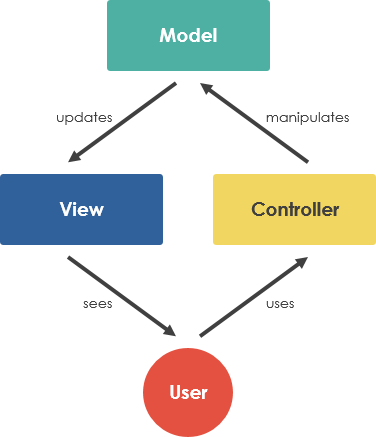
\includegraphics[scale=0.7]{slike/mvc-framework.PNG} 
			\centering
			\caption{MVC stil arhitekture}
			\label{mvc-framework}
		\end{figure}
	
		
		\section{Programski jezici, razvojni okviri, alati i biblioteke koda}
		
		
		\subsection{Back-end i baza podataka}
		U okviru \textit{back-end} aplikacije koriste se razni alati i tehnologije kako bi se postigla funkcionalnost web aplikacije. 
		
		Sama funkcionalnost \textit{back-enda} ostvarena je koristeći \textit{Kotlin} i \textit{Spring Boot}, popularne \textit{frameworke} za Javu i Kotlin.
		
		\textit{Spring Boot} olakšava izradu web aplikacije pružajući razne automatske konfiguracije. To uvelike omogućava integraciju različitih dijelova aplikacije i pruža mnogo gotovih implementacija koje se koriste putem vrlo intuitivnih sučelja.
		
		Baza podataka ostvarena je u \textit{PostgreSQL}-u, a za njenu jasnu definiciju korišten je alat \textit{Flyway}. \textit{Flyway} omogućava precizno i upravljivo definiranje strukture baze podataka.
		
		Za preslikavanje entiteta iz \textit{PostgreSQL} baze podataka u klase \textit{back-end} aplikacije korišten je \textit{JPA (Jakarta Persistence API)}, koji značajno olakšava generiranje upita ovisno o pozivima metoda nad klasama entiteta, a za komunikaciju baze i same aplikacije koristi se \textit{JDBC (Java Database Connectivity)}.
		
		Za konfiguracijske datoteke aplikacije koristi se \textit{YAML} format. Upravljanje bazom podataka odvija se preko \textit{Datagrip}-a, a razvoj kompletne \textit{back-end} aplikacije obavlja se u \textit{IntelliJ IDEA}, popularnom alatu tvrtke \textit{JetBrains}. 
		
		Za izgradnju cijele aplikacije koristi se \textit{Gradle}, alat za automatizaciju izgradnje. 
\textit{JWT (JSON Web Token}) standard korišten je za sigurnost aplikacije, generirajući tokene, koji istovremeno služe za autorizaciju i autentifikaciju korisnika.


			\subsection{Front-end}
			U izradi \textit{front-end} dijela aplikacije koristimo niz tehnologija kako bismo postigli željene funkcionalnosti i estetski privlačan dizajn. Ključne tehnologije koje se koriste u razvoju uključuju \textit{TypeScript}, \textit{React}, \textit{Bootstrap}, \textit{Vite} i \textit{IntelliJ}.
			
\textit{React}, kao glavni okvir, omogućava olakšanu izradu web stranica i pruža širok spektar alata za navigaciju, dohvaćanje i prikazivanje podataka. Koristi se označni kod sličan \textit{HTML}-u, obogaćen mogućnostima \textit{TypeScript}-a za definiranje sadržaja stranica, dok se za definiranje stila i izgleda koristi \textit{Bootstrap}.

Za efikasno upravljanje podacima u aplikaciji koristi se \textit{React Query}. \textit{Vite}, alat za brzu izgradnju aplikacija, osigurava optimiziran razvojni proces i ubrzanje vremena učitavanja stranica.

Konačno, za pisanje \textit{TypeScript} koda koristi se \textit{IntelliJ}, moćno razvojno okruženje koje omogućava precizno kodiranje i upravljanje projektom. Ovaj skup tehnologija omogućava nam izradu kvalitetne \textit{front-end} aplikacije s visokom funkcionalnošću i atraktivnim dizajnom.\\
		
		
				
		\section{Baza podataka}
			
		Između više tipova baza podataka (relacijska, hijerarhijska, objektno-orijentirana), za našu smo web aplikaciju odabrali koristiti relacijsku bazu podataka. Odlučili smo se za tu vrstu baze jer s njom imamo najviše iskustva, a jednostavna je, jasna i praktična za naše potrebe (upravljanje podacima o korisnicima koji postavljaju, izmjenjuju, brišu ili komentiraju oglase za izgubljene odnosno pronađene ljubimce) i implementaciju (klase u Springu su preslikane relacije iz baze) i omogućavaju jednostavan vizualni prikaz točnih međuovisnosti relacija, a time i veću razumljivost. Bazu podataka koristimo za efikasnu pohranu i dohvat podataka za obradu. Elementi baze podataka su relacije, odnosno tablice i njihovi vlastiti atributi. Baza podataka ove aplikacije sadrži 13 tablica:
		
		\begin{packed_item}
			\item User
			\item UserType
			\item Ad
			\item Activity
			\item Pet
			\item Color
			\item Of\_Color
			\item Species
			\item Message
			\item Image
			\item City
			\item County
			\item Location
		\end{packed_item}

			\subsection{Opis tablica}
			

				\textbf{APP\_USER} Predstavlja registriranog korisnika aplikacije, u \textit{@ManyToOne} vezi s \textbf{USER\_TYPE} preko \textit{userTypeId}.
				
				
				\begin{longtblr}[
					label=none,
					entry=none
					]{
						width = \textwidth,
						colspec={|X[8,l]|X[6, l]|X[18, l]|}, 
						rowhead = 1,
					}
					\hline \SetCell[c=3]{c}{\textbf{APP\_USER}}	 \\ \hline[3pt]
					\SetCell{LightGreen}userId & BIGINT	&  	jedinstveni ID korisnika  	\\ \hline
					username	& VARCHAR &   korisničko ime (jedinstveno)	\\ \hline 
					email & VARCHAR &   korisnikova e-mail adresa (jedinstvena)	\\ \hline 
					password & VARCHAR	&  	korisnikova lozinka	\\ \hline 
					name & VARCHAR	&  	ime korisnika	\\ \hline 
					telephone\_number & VARCHAR	&  	korisnikov broj telefona (jedinstven)	\\ \hline 
					\SetCell{LightBlue} userTypeId	& BIGINT &   ID koji označava tip korisnika	\\ \hline 
				\end{longtblr}
				
				\noindent\textbf{USER\_TYPE} Predstavlja popis tipova korisnika aplikacije (userTypeId=1 odgovara osobi, userTypeId=2 skloništu).
				
				
				\begin{longtblr}[
					label=none,
					entry=none
					]{
						width = \textwidth,
						colspec={|X[8,l]|X[6, l]|X[18, l]|}, 
						rowhead = 1,
					}
					\hline \SetCell[c=3]{c}{\textbf{USER\_TYPE}}	 \\ \hline[3pt]
					\SetCell{LightGreen}userTypeId & BIGINT	&  	jedinstveni ID tipa korisnika  	\\ \hline
					name	& VARCHAR &   ime tipa korisnika	\\ \hline 
				\end{longtblr}
				
				\noindent\textbf{MESSAGE} Poruka koju korisnici mogu ostavljati u komunikaciji ispod oglasa, u \textit{@ManyToOne} vezi s \textbf{AD} preko \textit{adId}, \textit{@ManyToOne} vezi s \textbf{USER} preko \textit{userId}, \textit{@OneToOne} vezi s \textbf{LOCATION} preko \textit{locationId}.
				
				\begin{longtblr}[
					label=none,
					entry=none
					]{
						width = \textwidth,
						colspec={|X[8,l]|X[6, l]|X[18, l]|}, 
						rowhead = 1,
					}
					\hline \SetCell[c=3]{c}{\textbf{MESSAGE}}	 \\ \hline[3pt]
					\SetCell{LightGreen}messageId & BIGINT	&  	jedinstveni ID poruke  	\\ \hline
					text	& VARCHAR &   sadržaj poruke	\\ \hline 
					date	& DATE &   datum kada je poruka ostavljena ispod oglasa	\\ \hline 
					\SetCell{LightBlue}adId	& BIGINT &   jedinstveni ID oglasa ispod kojeg je poruka ostavljena	\\ \hline 
					\SetCell{LightBlue}locationId	& BIGINT &   jedinstveni ID lokacije 	\\ \hline 
					\SetCell{LightBlue}userId	& BIGINT &   jedinstveni ID korisnika koji je ostavio poruku	\\ \hline 
				\end{longtblr}
				
				\noindent\textbf{IMAGE} Tablica u koju se spremaju slike koje se dohvaćaju preko URL.
				
				\begin{longtblr}[
					label=none,
					entry=none
					]{
						width = \textwidth,
						colspec={|X[8,l]|X[6, l]|X[18, l]|}, 
						rowhead = 1,
					}
					\hline \SetCell[c=3]{c}{\textbf{IMAGE}}	 \\ \hline[3pt]
					\SetCell{LightGreen}imageId & BIGINT	&  	jedinstveni ID slike  	\\ \hline
					imageUrl	& VARCHAR &   URL slike	\\ \hline 
					\SetCell{LightBlue}adId & BIGINT	&  	jedinstveni ID pripadajućeg oglasa  	\\ \hline
					\SetCell{LightBlue}messageId & BIGINT	&  	jedinstveni ID pripadajuće poruke  	\\ \hline
				\end{longtblr}
				
				\noindent\textbf{ACTIVITY} Predstavlja kategoriju oglasa.
				
				\begin{longtblr}[
					label=none,
					entry=none
					]{
						width = \textwidth,
						colspec={|X[8,l]|X[6, l]|X[18, l]|}, 
						rowhead = 1,
					}
					\hline \SetCell[c=3]{c}{\textbf{ACTIVITY}}	 \\ \hline[3pt]
					\SetCell{LightGreen}activityId & BIGINT	&  	jedinstveni ID kategorije  	\\ \hline
					activityCategory	& VARCHAR &   naziv kategorije	\\ \hline 
				\end{longtblr}
				
				\noindent\textbf{AD} Predstavlja oglas, u \textit{@ManyToOne} vezi s \textbf{ACTIVITY}, \textit{@ManyToOne} vezi s \textbf{USER} preko \textit{userId}, \textit{@OneToOne} vezi s \textbf{PET}.
				
				\begin{longtblr}[
					label=none,
					entry=none
					]{
						width = \textwidth,
						colspec={|X[8,l]|X[6, l]|X[18, l]|}, 
						rowhead = 1,
					}
					\hline \SetCell[c=3]{c}{\textbf{AD}}	 \\ \hline[3pt]
					\SetCell{LightGreen}adId & BIGINT	&  	jedinstveni ID oglasa  	\\ \hline
					inShelter	& INT &   1 ako je oglas od skloništa, inače 0 	\\ \hline 
					deleted	& INT &   1 ako je oglas obrisan, inače 0 	\\ \hline 
					\SetCell{LightBlue}activityId	& BIGINT &   jedinstveni ID kategorije oglasa 	\\ \hline
					\SetCell{LightBlue}petId	& BIGINT &   jedinstveni ID ljubimca u oglasu 	\\ \hline
					\SetCell{LightBlue}userId	& BIGINT &   jedinstveni ID korisnika koji je postavio oglas 	\\ \hline 
				\end{longtblr}
				
				\noindent\textbf{PET} Predstavlja ljubimca, u \textit{@ManyToMany} vezi s \textbf{COLOR}, \textit{@ManyToOne} vezi sa \textbf{SPECIES}, \textit{@OneToOne} vezi s \textbf{LOCATION}.
				
				\begin{longtblr}[
					label=none,
					entry=none
					]{
						width = \textwidth,
						colspec={|X[8,l]|X[6, l]|X[18, l]|}, 
						rowhead = 1,
					}
					\hline \SetCell[c=3]{c}{\textbf{PET}}	 \\ \hline[3pt]
					\SetCell{LightGreen}petId & BIGINT	&  	jedinstveni ID ljubimca  	\\ \hline
					petName	& VARCHAR &   ime na koje se ljubimac odaziva	\\ \hline 
					petAge	& INT &   starost ljubimca	\\ \hline 
					dateTimeMissing	& DATETIME &   datum i vrijeme nestanka ljubimca	\\ \hline 
					description	& VARCHAR &   opis ljubimca	\\ \hline 
					\SetCell{LightBlue}speciesId	& BIGINT &   jedinstveni ID vrste ljubimca	\\ \hline 
					\SetCell{LightBlue}locationId	& BIGINT &   ID lokacije nestanka ljubimca	\\ \hline 
				\end{longtblr}
				
				\noindent\textbf{SPECIES} Tablica vrsta ljubimaca.
				
				\begin{longtblr}[
					label=none,
					entry=none
					]{
						width = \textwidth,
						colspec={|X[8,l]|X[6, l]|X[18, l]|}, 
						rowhead = 1,
					}
					\hline \SetCell[c=3]{c}{\textbf{SPECIES}}	 \\ \hline[3pt]
					\SetCell{LightGreen}speciesId & BIGINT	&  	jedinstveni ID vrste ljubimca  	\\ \hline
					speciesName	& VARCHAR &   naziv vrste ljubimca	\\ \hline 
				\end{longtblr}
				
				\noindent\textbf{COLOR} Tablica s bojama ljubimaca, u \textit{@ManyToMany} vezi s \textbf{PET}.
				
				\begin{longtblr}[
					label=none,
					entry=none
					]{
						width = \textwidth,
						colspec={|X[8,l]|X[6, l]|X[18, l]|}, 
						rowhead = 1,
					}
					\hline \SetCell[c=3]{c}{\textbf{COLOR}}	 \\ \hline[3pt]
					\SetCell{LightGreen}colorId & BIGINT	&  	jedinstveni ID boje  	\\ \hline
					colorName	& VARCHAR &   naziv boje	\\ \hline 
				\end{longtblr}
				
				\noindent\textbf{OF\_COLOR} Tablica veze između \textbf{PET} i \textbf{COLOR}.
				
				\begin{longtblr}[
					label=none,
					entry=none
					]{
						width = \textwidth,
						colspec={|X[8,l]|X[6, l]|X[18, l]|}, 
						rowhead = 1,
					}
					\hline \SetCell[c=3]{c}{\textbf{OF\_COLOR}}	 \\ \hline[3pt]
					\SetCell{LightBlue}colorId & BIGINT	&  	jedinstveni ID boje  	\\ \hline
					\SetCell{LightBlue}petId & BIGINT	&  	jedinstveni ID ljubimca	\\ \hline
				\end{longtblr}
				
				\noindent\textbf{COUNTY} Predstavlja županije nestanka/pronalaska ljubimaca.
				
				\begin{longtblr}[
					label=none,
					entry=none
					]{
						width = \textwidth,
						colspec={|X[8,l]|X[6, l]|X[18, l]|}, 
						rowhead = 1,
					}
					\hline \SetCell[c=3]{c}{\textbf{COUNTY}}	 \\ \hline[3pt]
					\SetCell{LightGreen}countyId & BIGINT	&  	jedinstveni ID županije  	\\ \hline
					countyName & VARCHAR	&  	naziv županije	\\ \hline
				\end{longtblr}
				
				\noindent\textbf{CITY} Predstavlja gradove nestanka/pronalaska ljubimaca, u \textit{@ManyToOne} vezi s \textbf{COUNTY}.
				
				\begin{longtblr}[
					label=none,
					entry=none
					]{
						width = \textwidth,
						colspec={|X[8,l]|X[6, l]|X[18, l]|}, 
						rowhead = 1,
					}
					\hline \SetCell[c=3]{c}{\textbf{CITY}}	 \\ \hline[3pt]
					\SetCell{LightGreen}cityId & BIGINT	&  	jedinstveni ID grada  	\\ \hline
					cityName & VARCHAR	&  	naziv grada	\\ \hline
					\SetCell{LightBlue}countyId & BIGINT	&  	jedinstveni ID županije  	\\ \hline
					
				\end{longtblr}
				
				\noindent\textbf{LOCATION} Predstavlja točne lokacije, u \textit{@ManyToOne} vezi sa \textbf{CITY}.
				
				\begin{longtblr}[
					label=none,
					entry=none
					]{
						width = \textwidth,
						colspec={|X[8,l]|X[6, l]|X[18, l]|}, 
						rowhead = 1,
					}
					\hline \SetCell[c=3]{c}{\textbf{LOCATION}}	 \\ \hline[3pt]
					\SetCell{LightGreen}locationId & BIGINT	&  	jedinstveni ID lokacije  	\\ \hline
					longitude & DOUBLE PRECISION	&  	geografska dužina	\\ \hline
					latitude & DOUBLE PRECISION	&  	geografska širina	\\ \hline
					\SetCell{LightBlue}cityId & BIGINT	&  	jedinstveni ID grada  	\\ \hline
					
				\end{longtblr}
				
			
			\subsection{Dijagram baze podataka}
			\begin{figure}[H]
				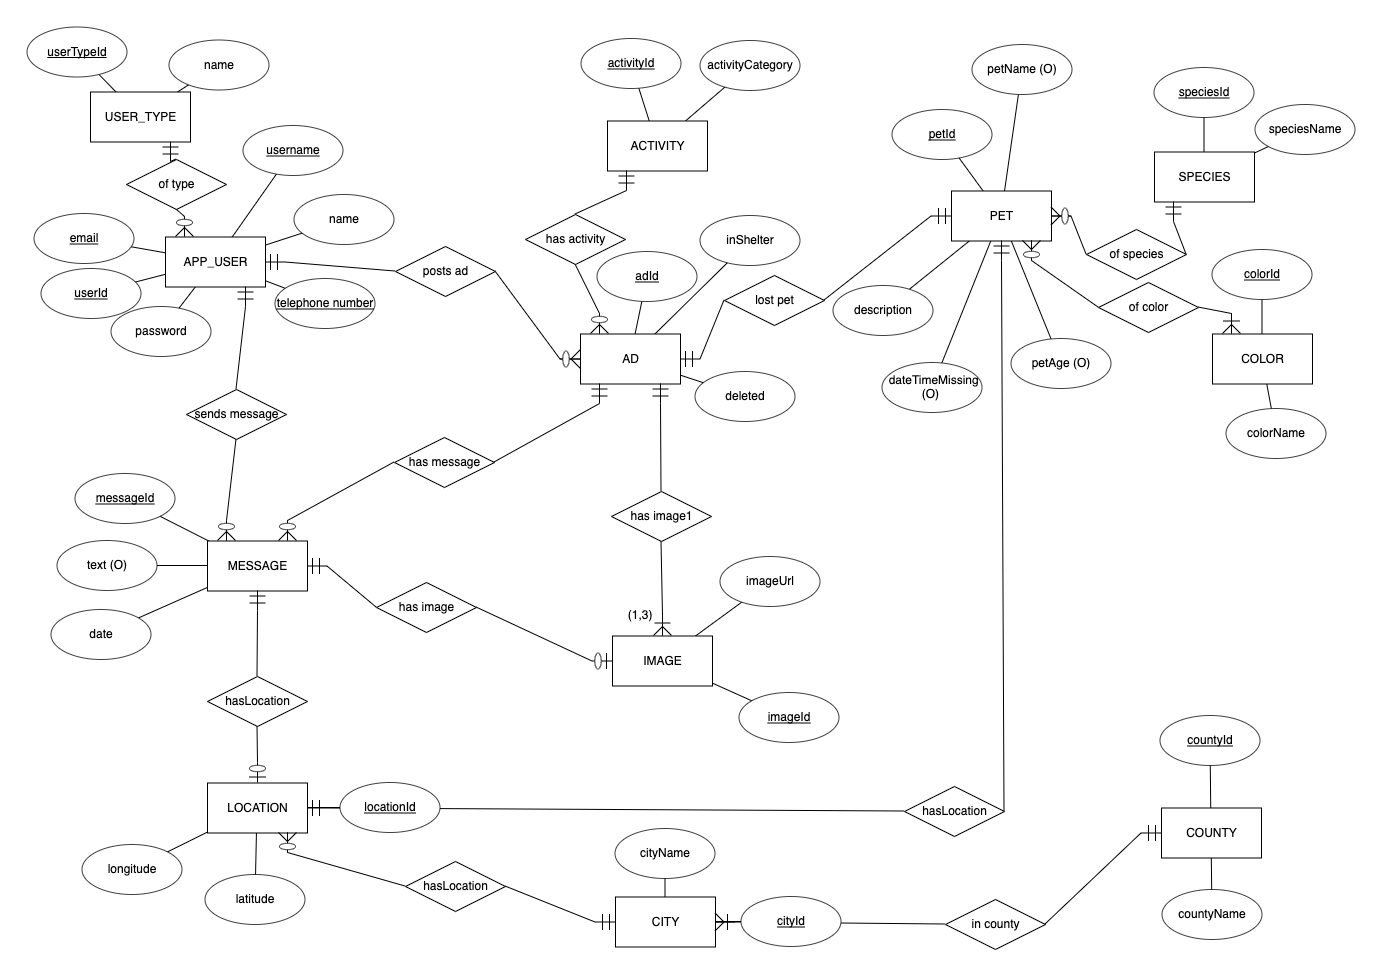
\includegraphics[scale=0.33]{slike/ER_DIAGRAM_FINAL.PNG} 
				\centering
				\caption{ER dijagram baze podataka}
				\label{ER_diagram}
			\end{figure}
			
			\begin{figure}[H]
				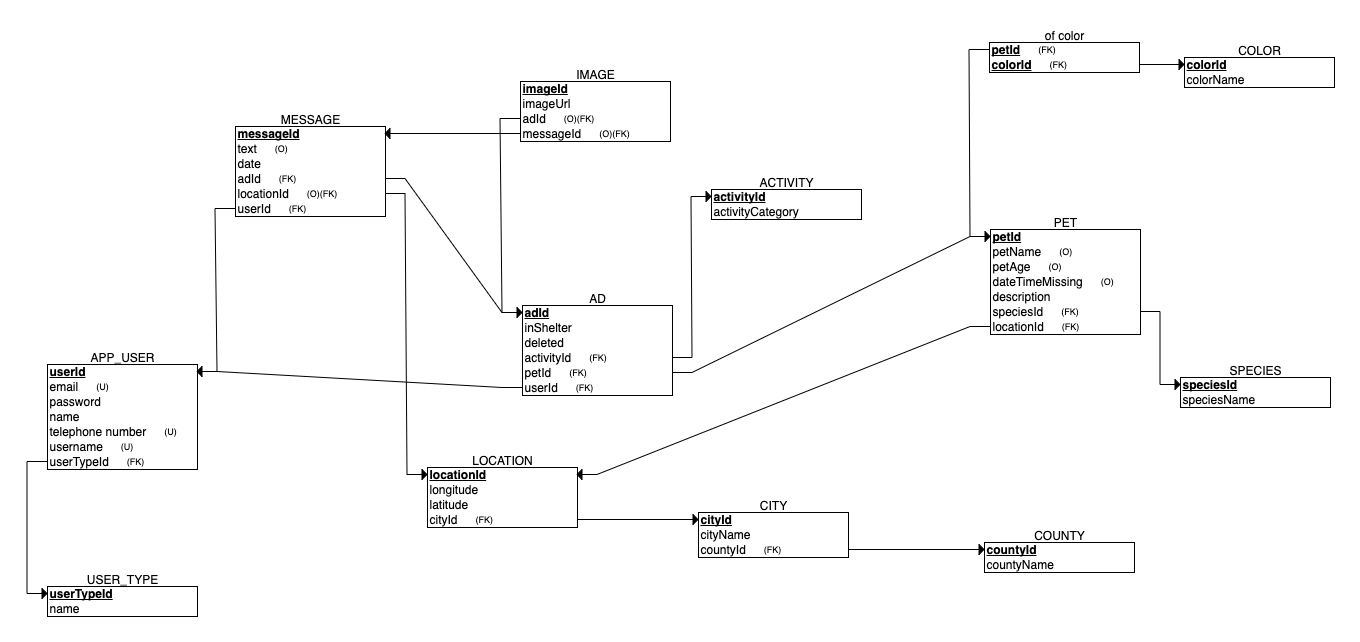
\includegraphics[scale=0.34]{slike/REL_DIAGRAM_FINAL.PNG} 
				\centering
				\caption{Relacijski dijagram baze podataka}
				\label{relational_diagram}
			\end{figure}
			
			\eject
			
			
		\section{Dijagram razreda}

			Na dijagramima su prikazani razredi vezani uz serversku stranu aplikacije.
			
			Dijagram na slici \ref{class_model} prikazuje razrede entitete (modele) koji odgovaraju tablicama u bazi podataka.
			
			\begin{figure}[H]
				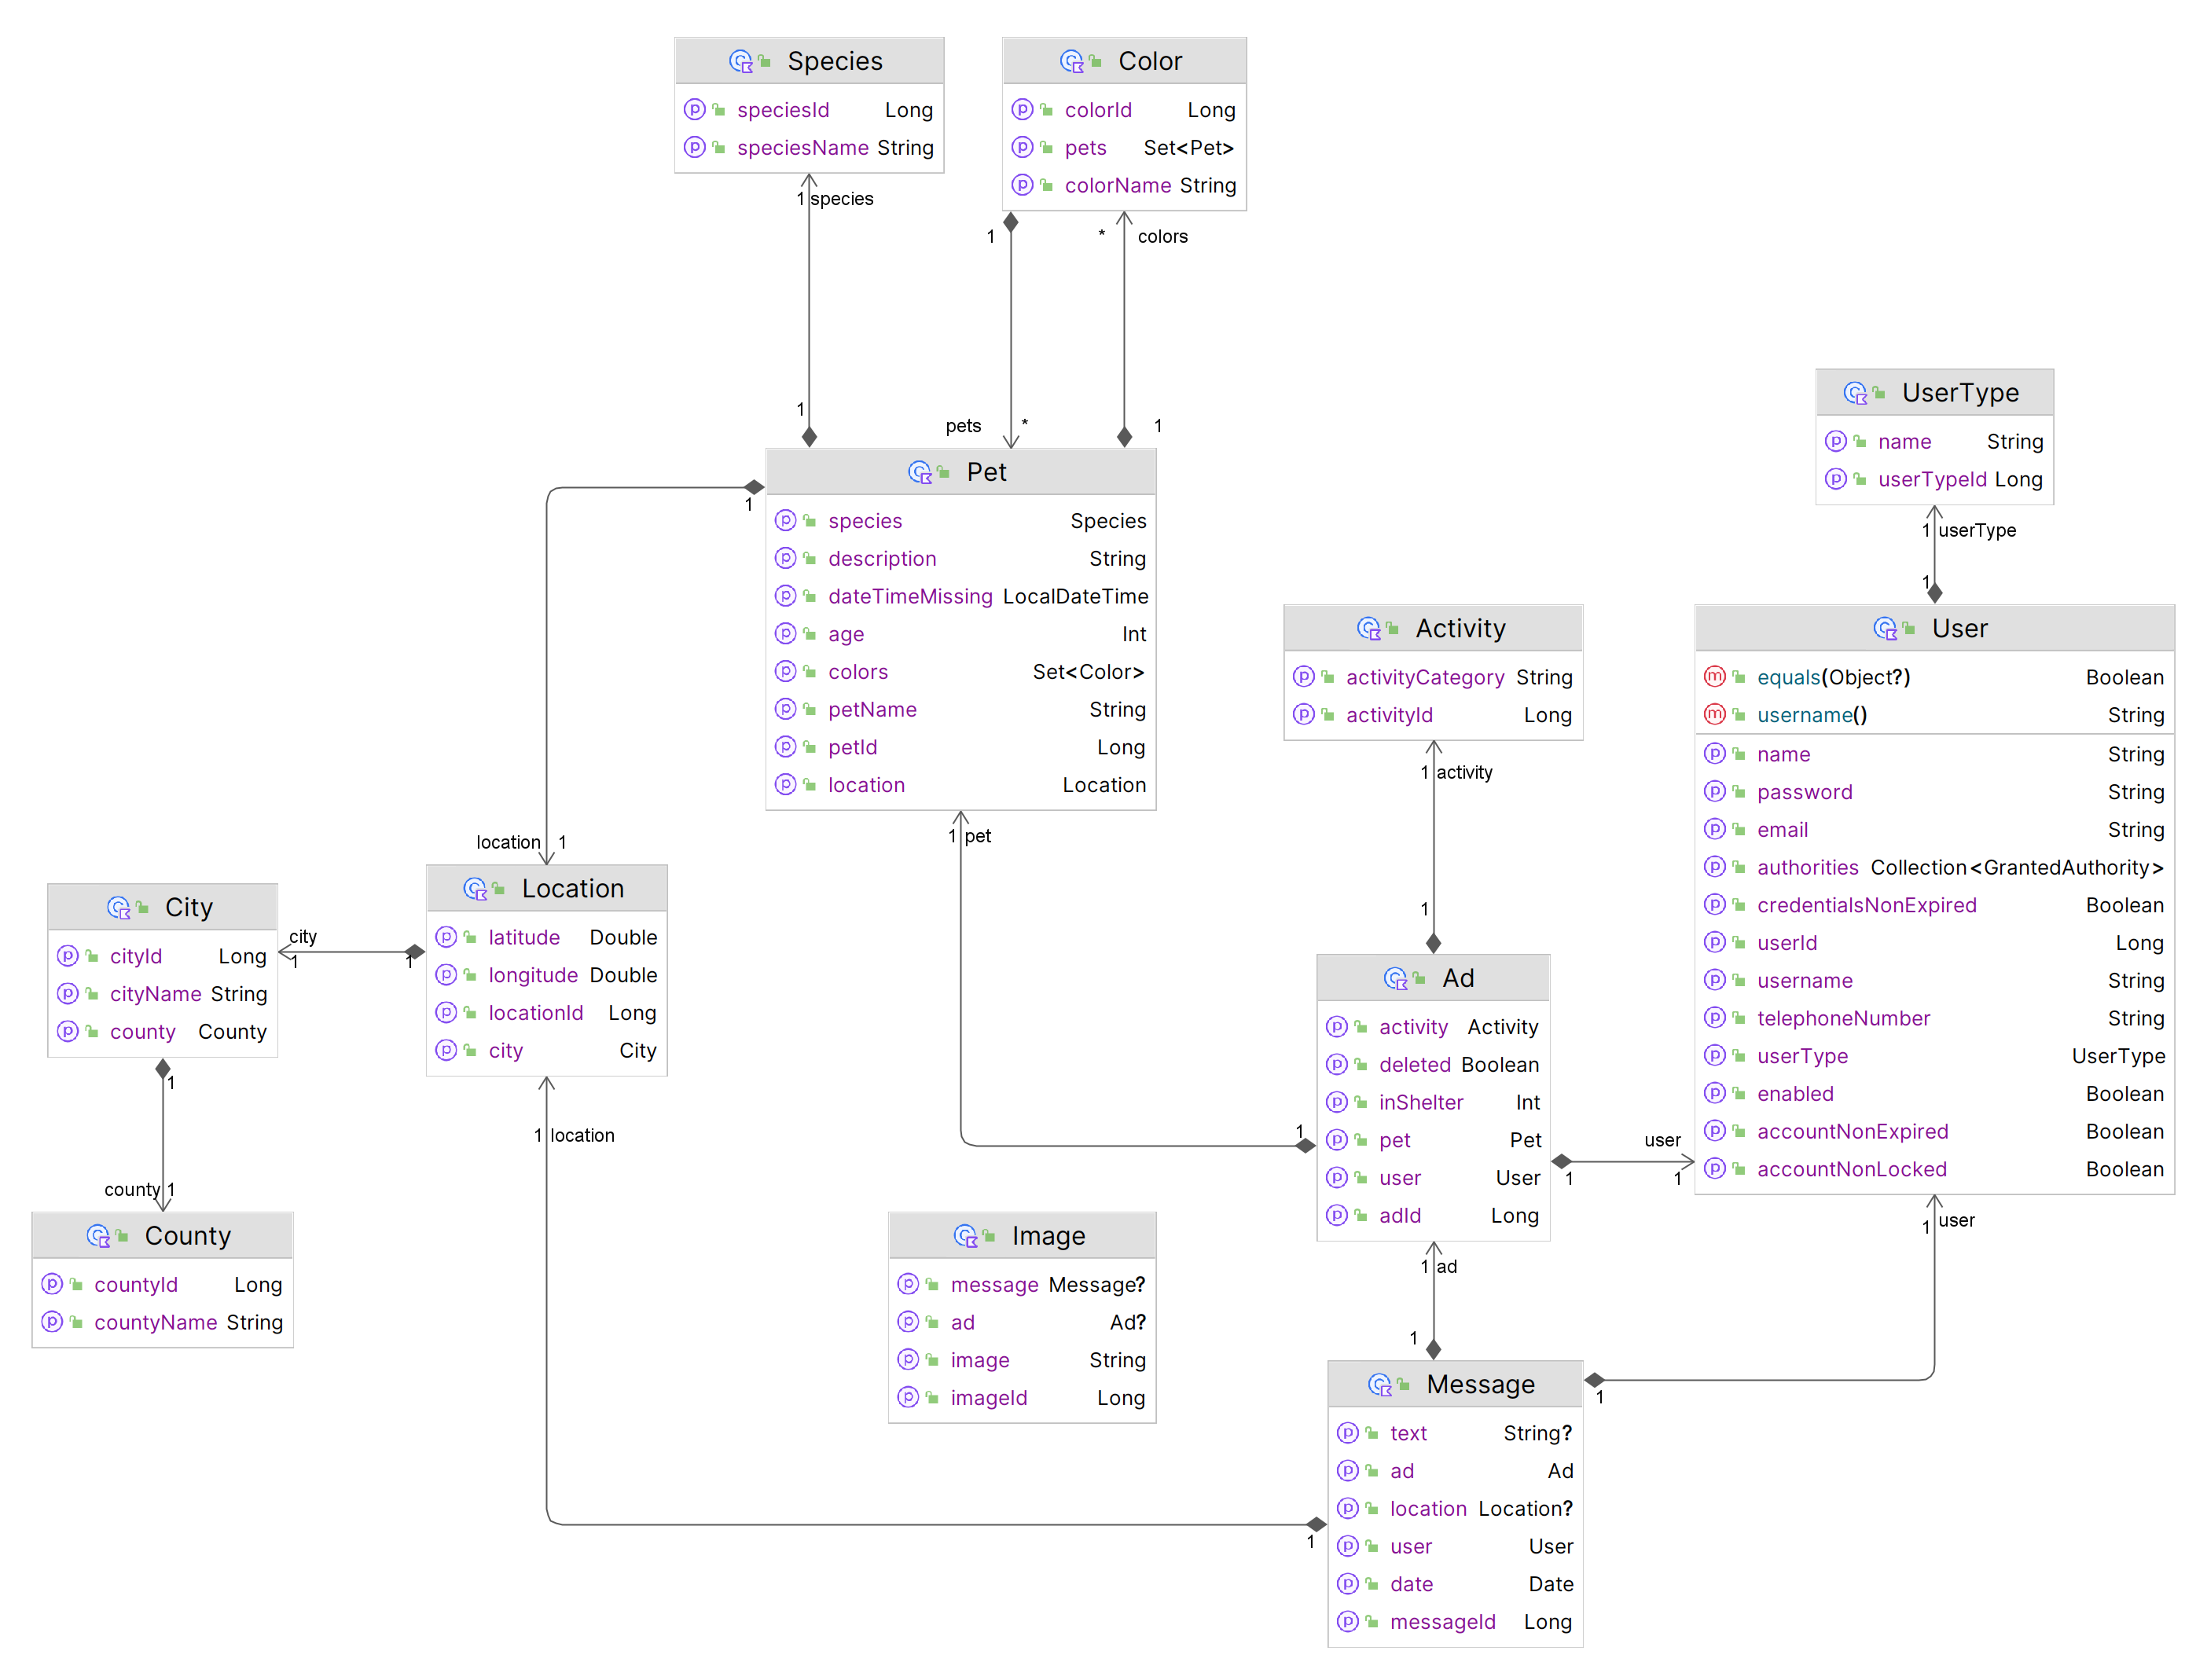
\includegraphics[scale=0.225]{slike/class_model.PNG} 
				\centering
				\caption{Dijagram razreda entiteta}
				\label{class_model}
			\end{figure}
			
			Na slici \ref{class_repo} prikazana su sučelja \textit{Repository} (npr. UserRepository, MessageRepository), odgovorna za komuniciranje s bazom podataka. Radi preglednosti je na slici \ref{class_service_repo} prikazan samo odnos UserService i UserRepository, ostali se ponašaju analogno.
			
			\begin{figure}[H]
				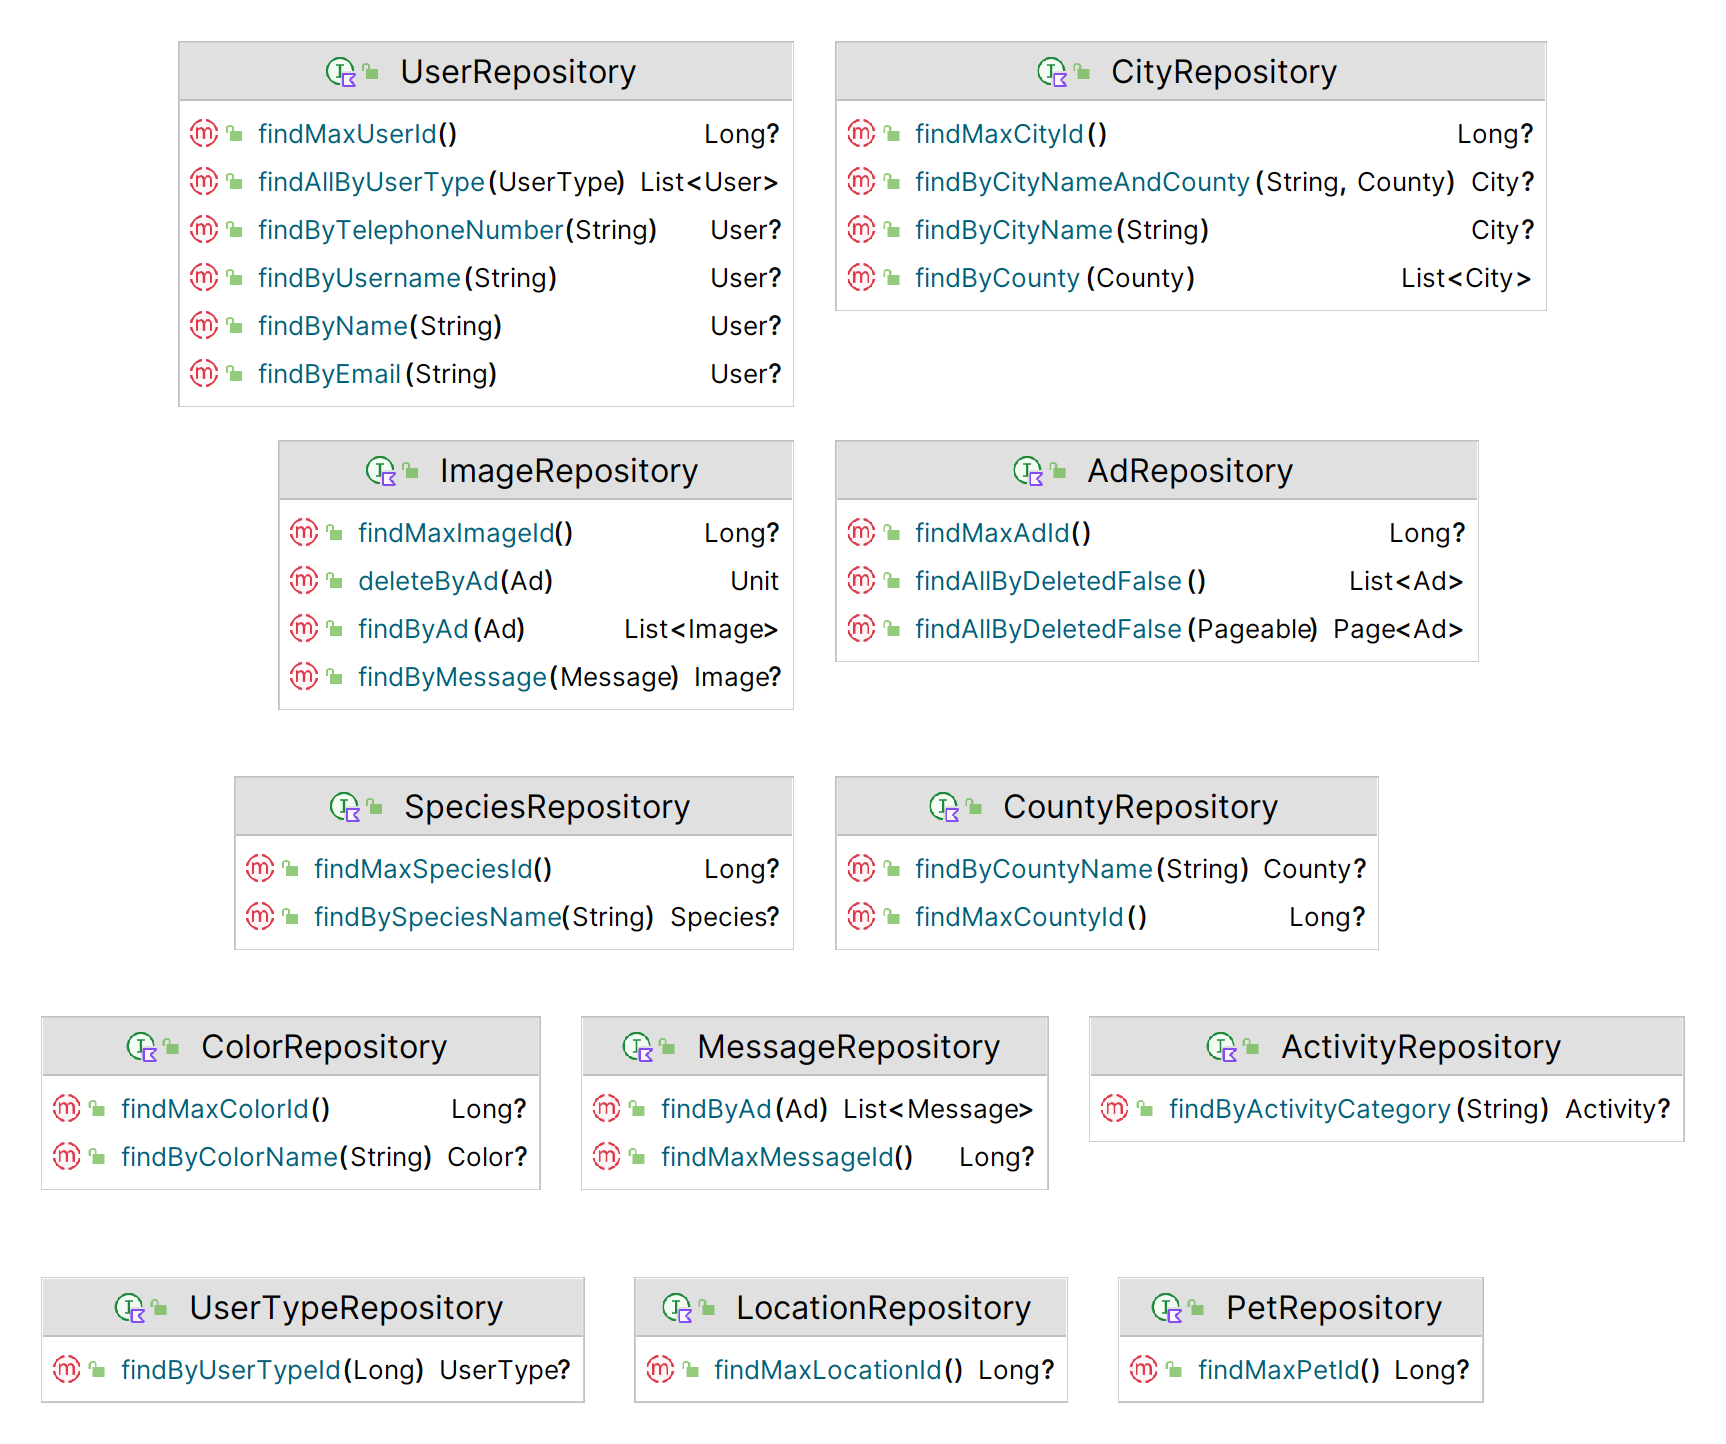
\includegraphics[scale=0.25]{slike/class_repo.PNG} 
				\centering
				\caption{Dijagram razreda \textit{Repository}}
				\label{class_repo}
			\end{figure}
			
			\begin{figure}[H]
				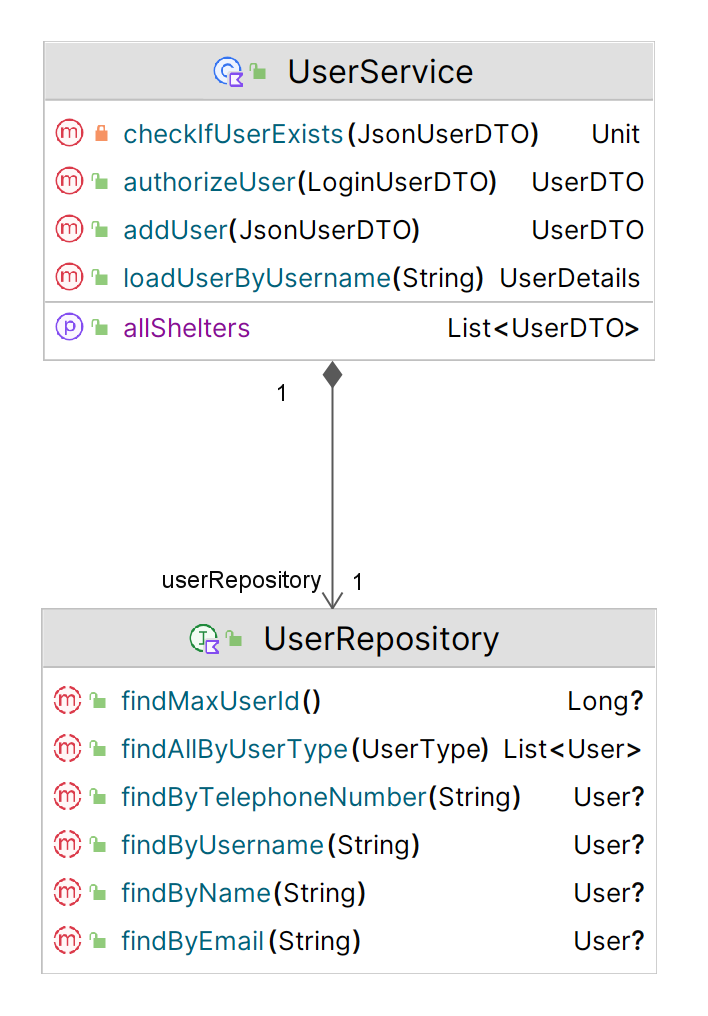
\includegraphics[scale=0.35]{slike/class_service_repo.PNG} 
				\centering
				\caption{UserService i UserRepository}
				\label{class_service_repo}
			\end{figure}
			
			Dijagrami \ref{class_ad}, \ref{class_add_ad_message}, \ref{class_message}, \ref{class_user}, \ref{class_city_county}, \ref{class_species_color} prikazuju odnose između \textit{Controller}, \textit{Service} i \textit{Data Transfer Object} (DTO) razreda vezanih uz oglase, poruke, korisnike, gradove i županije te boje i vrste ljubimaca.
			
			\begin{figure}[H]
				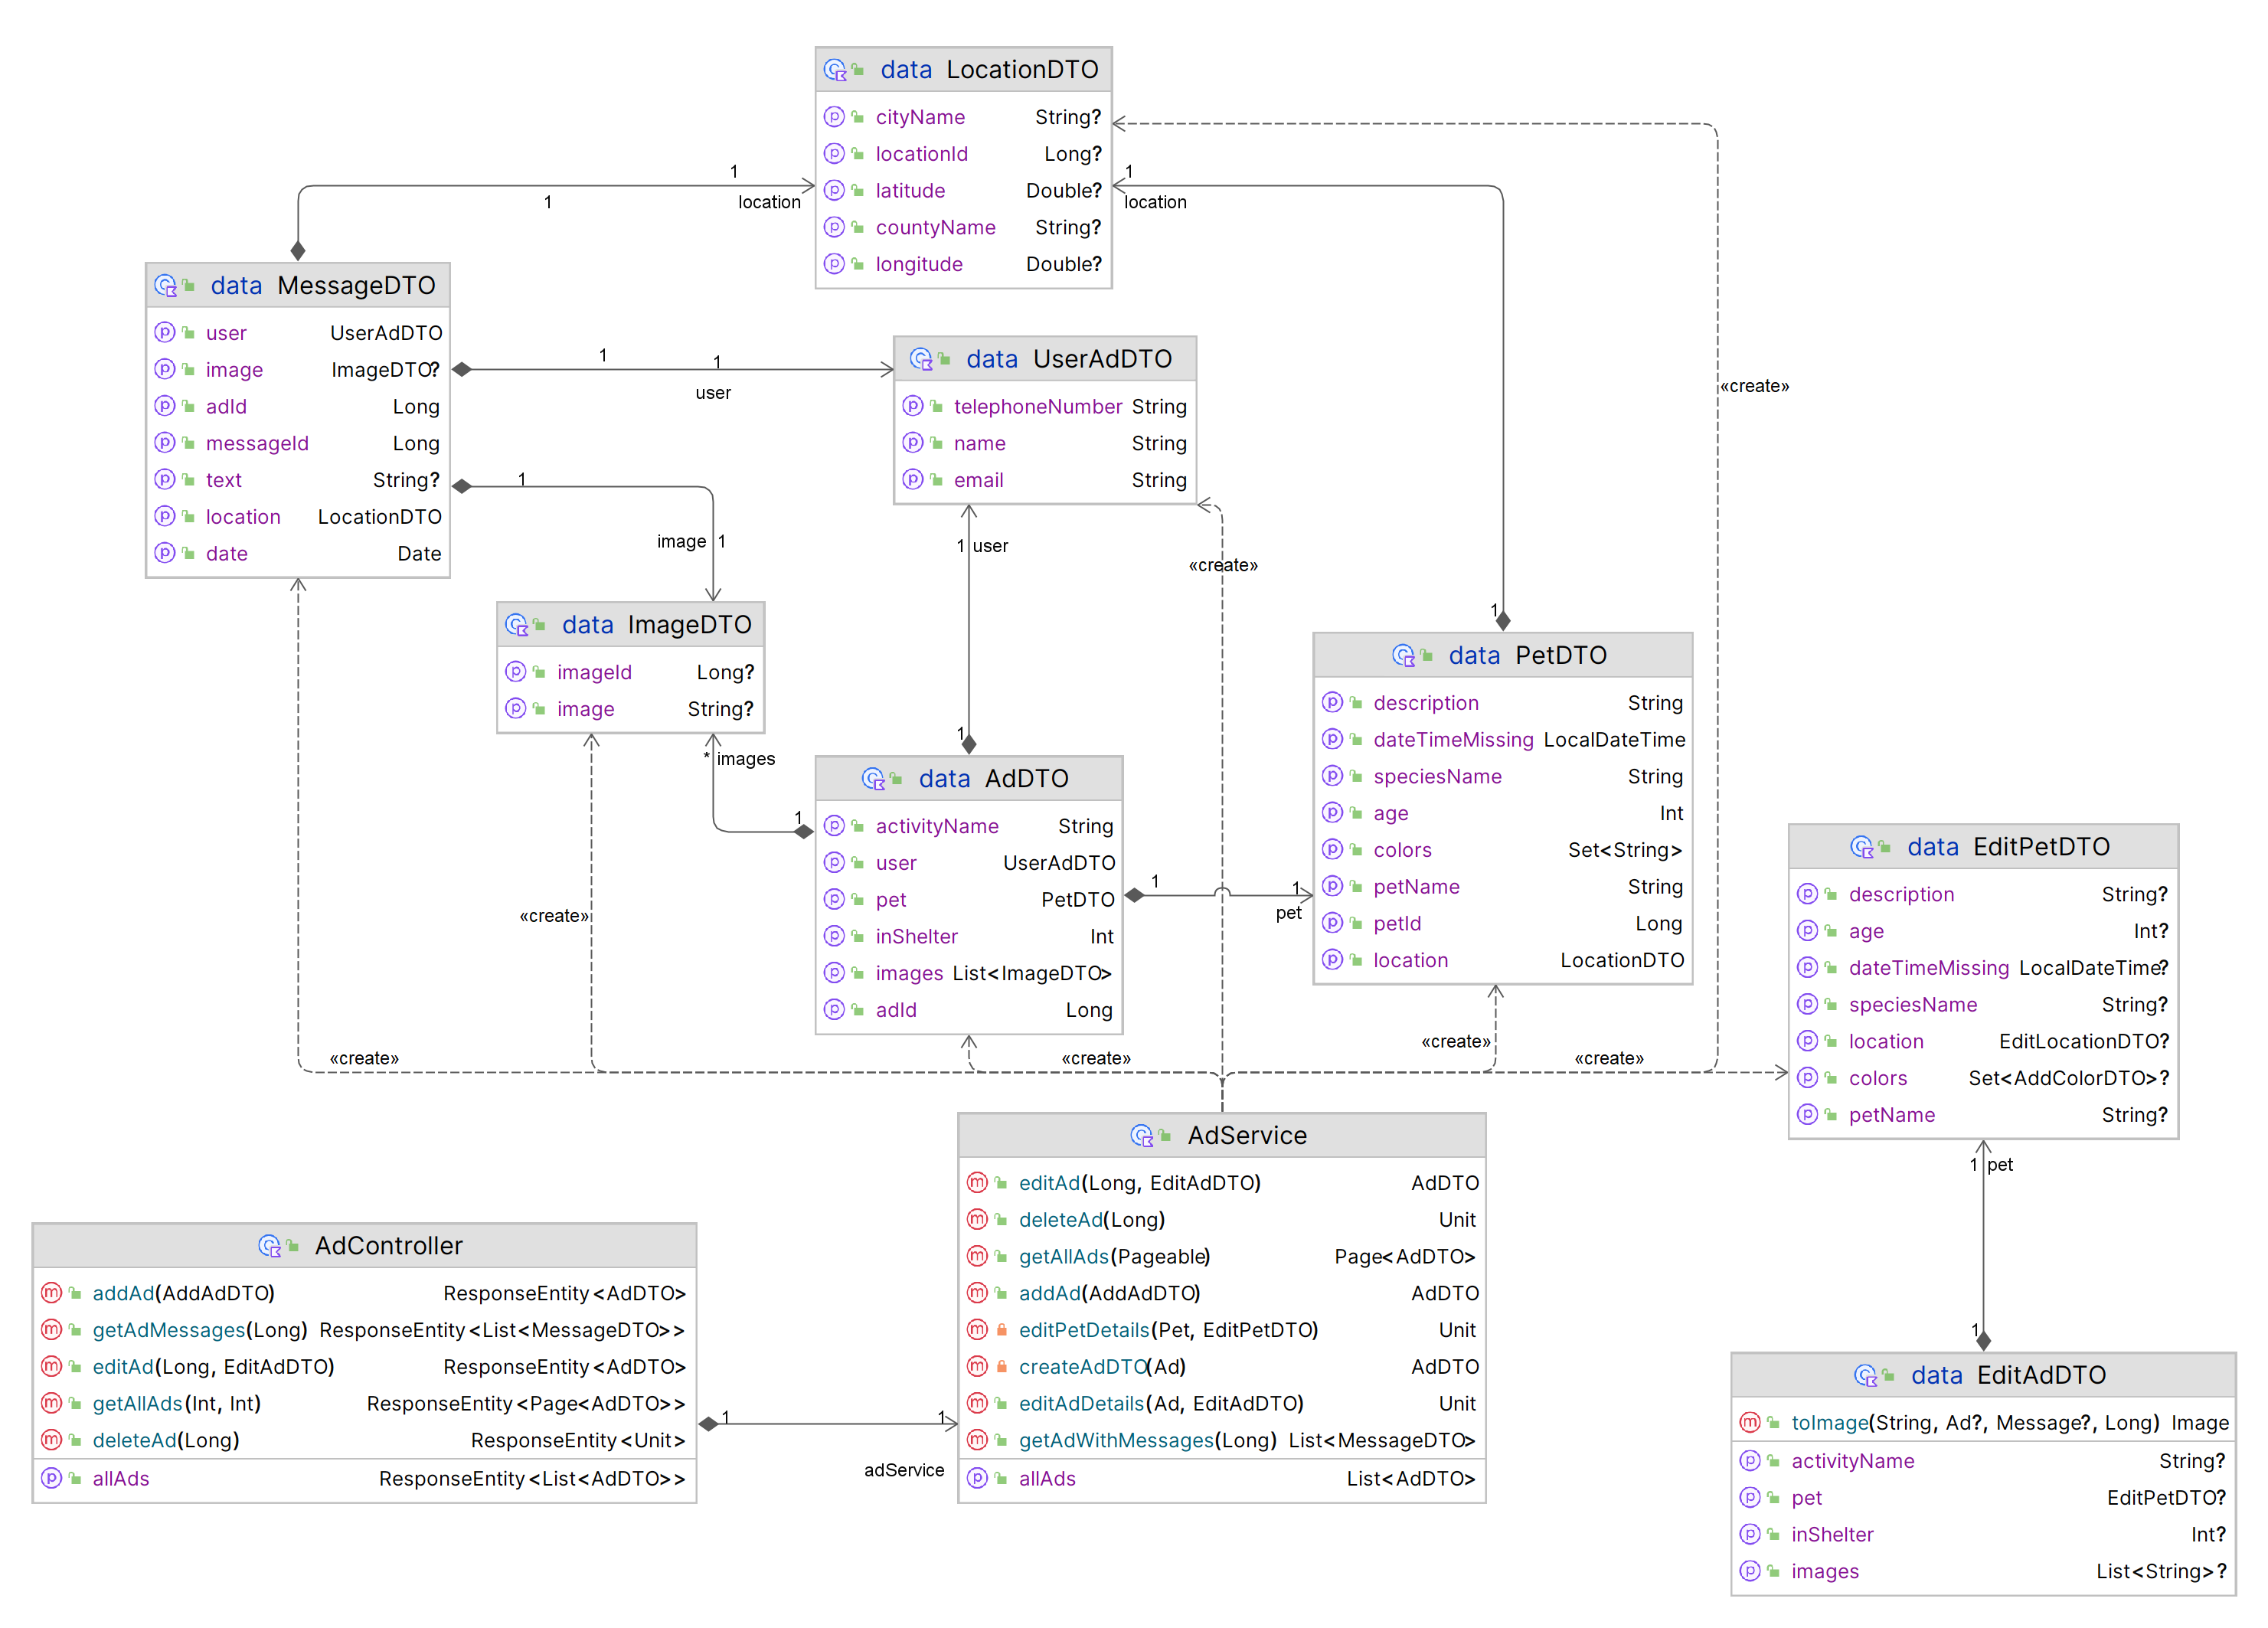
\includegraphics[scale=0.225]{slike/class_ad.PNG} 
				\centering
				\caption{Razredi - oglasi}
				\label{class_ad}
			\end{figure}
			
			\begin{figure}[H]
				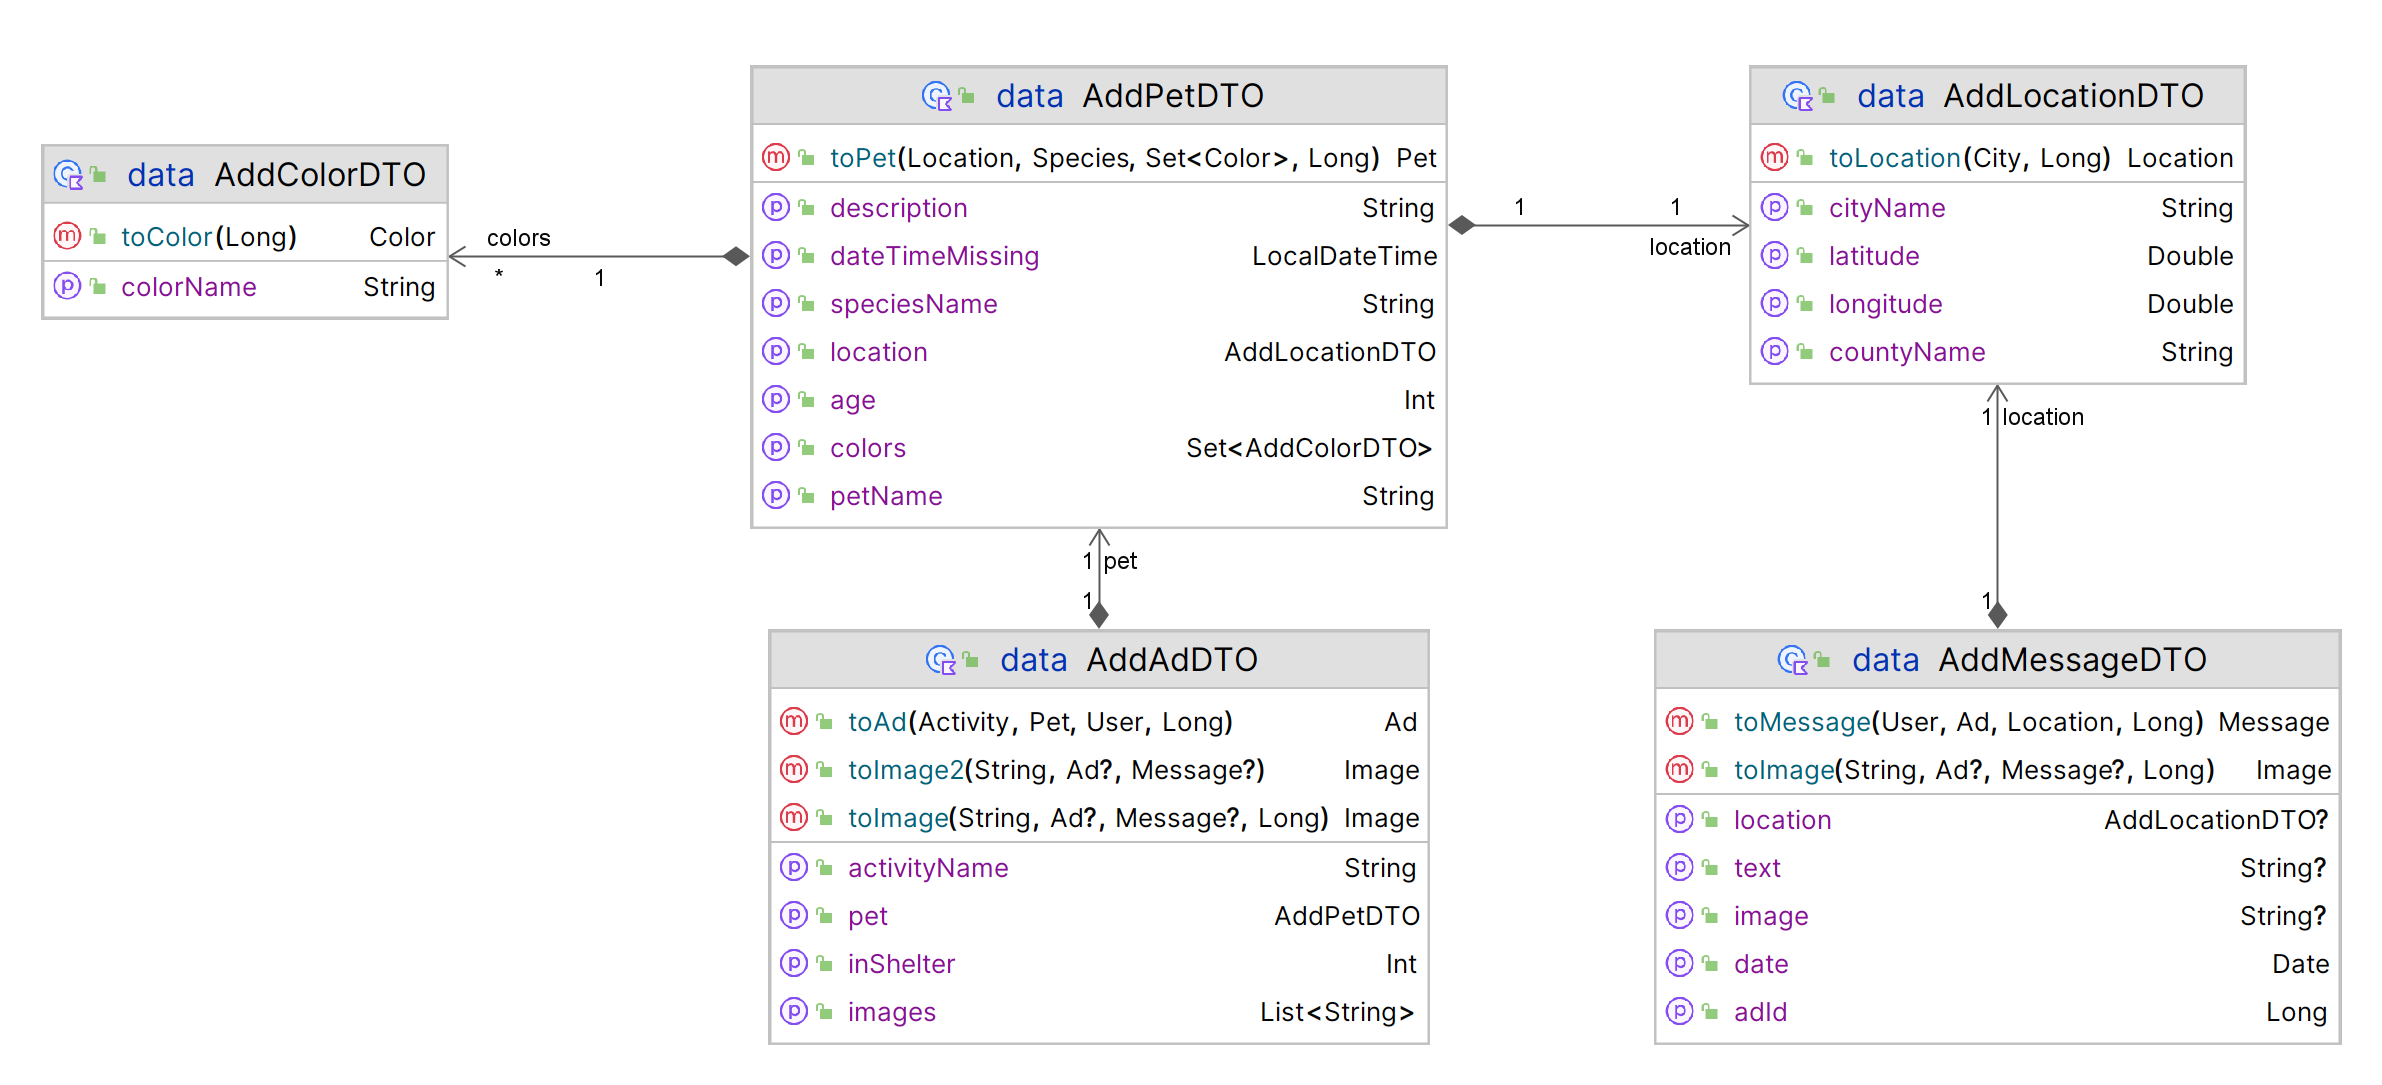
\includegraphics[scale=0.25]{slike/class_add_ad_message.PNG} 
				\centering
				\caption{Razredi - dodavanje oglasa i poruka}
				\label{class_add_ad_message}
			\end{figure}
			
			\begin{figure}[H]
				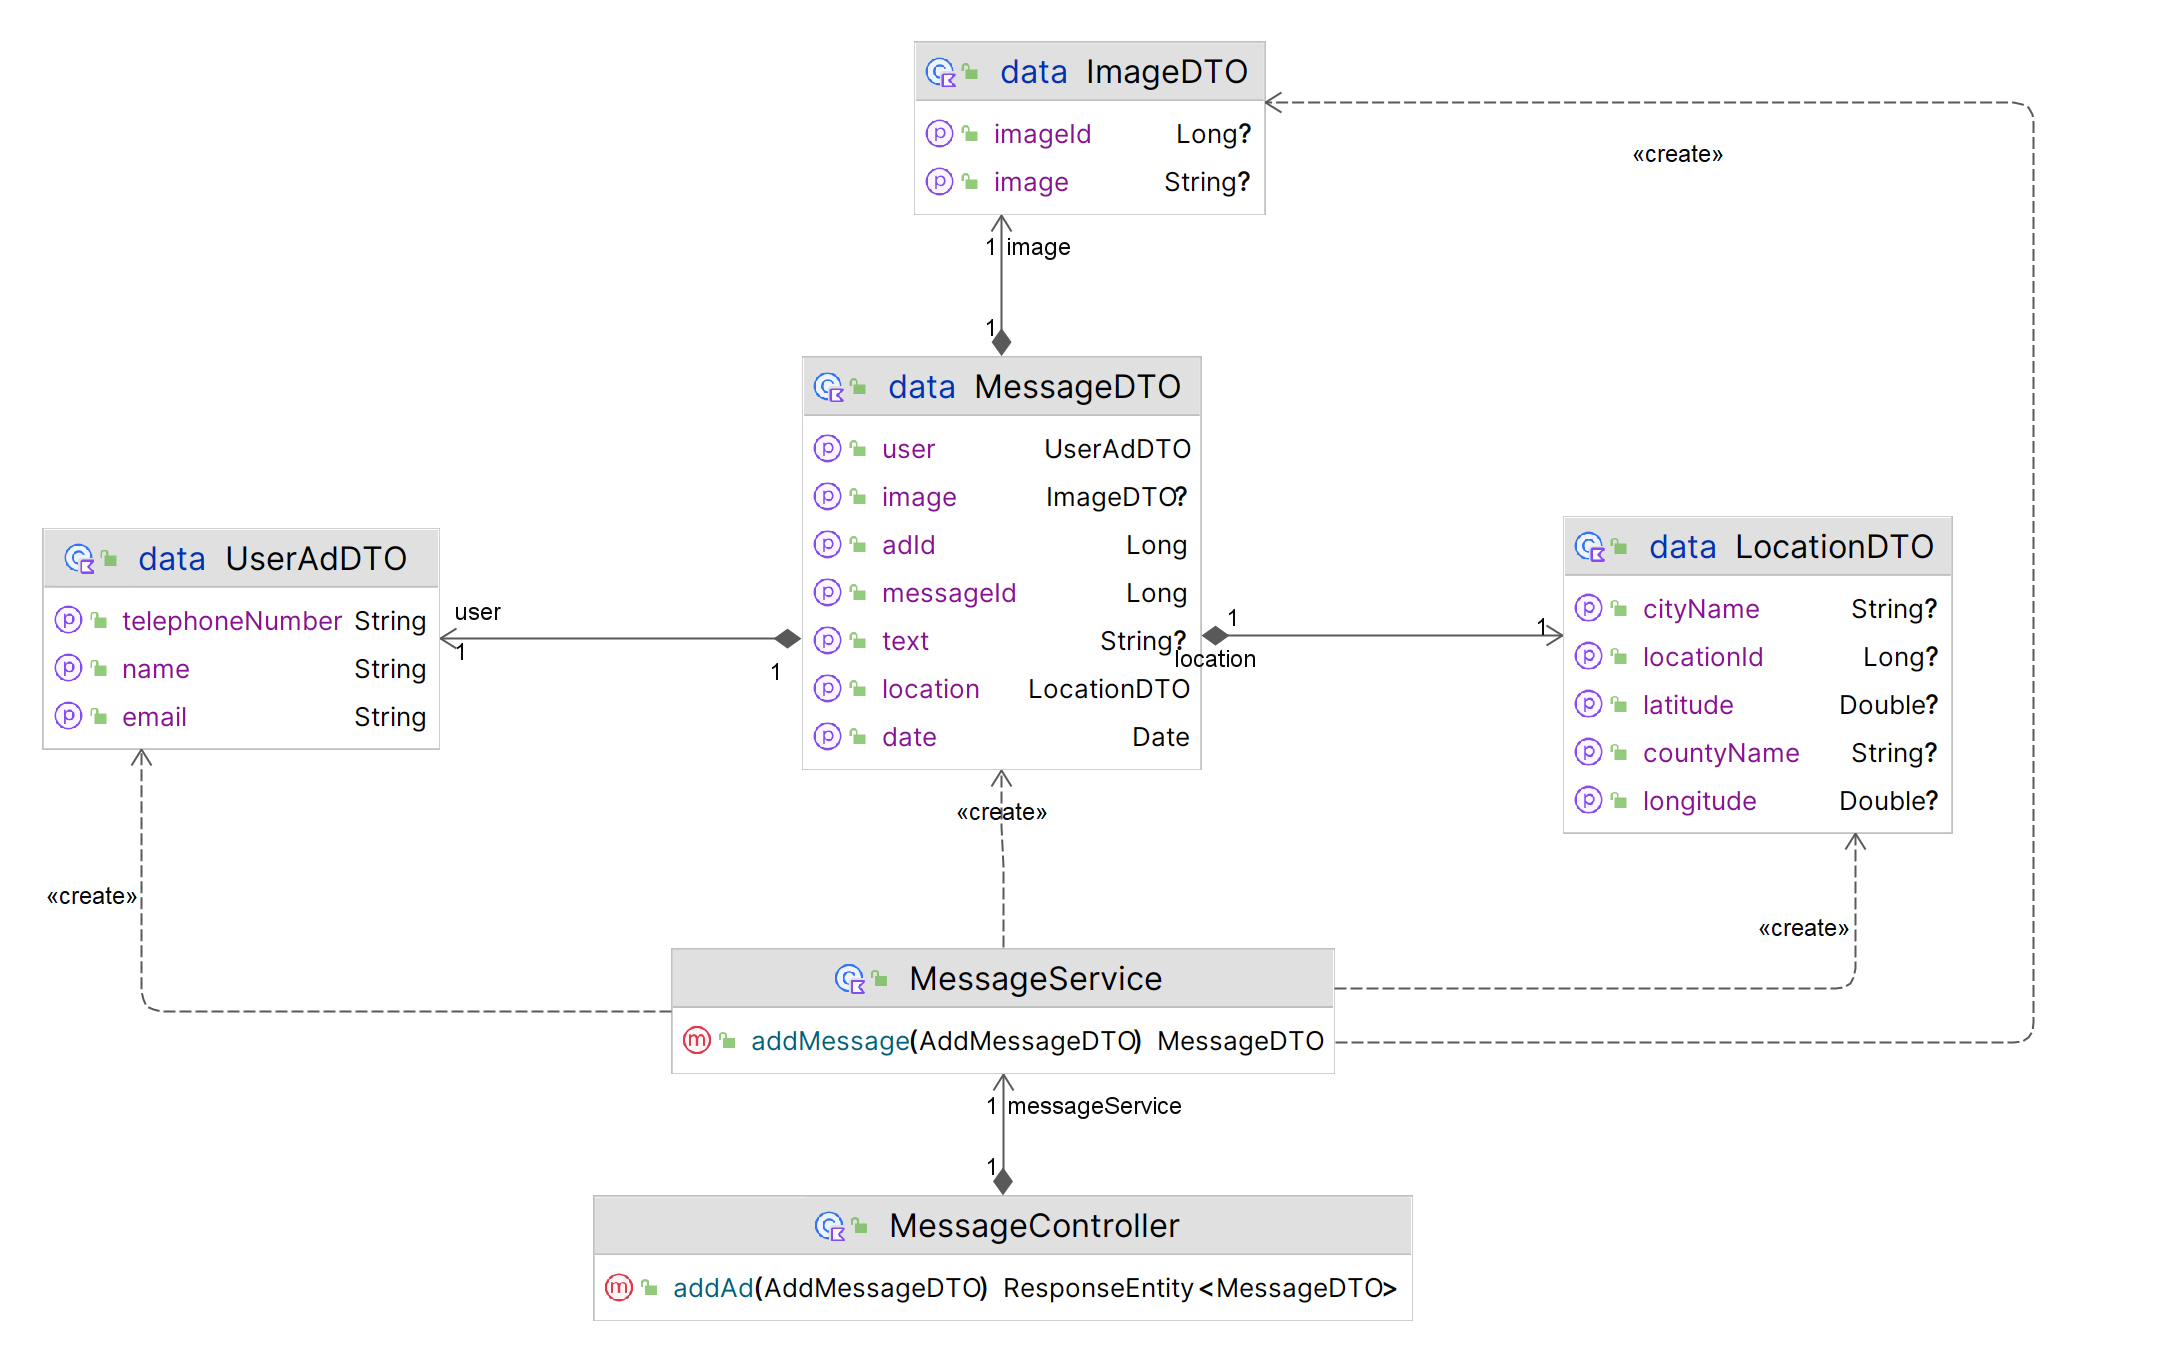
\includegraphics[scale=0.25]{slike/class_message.PNG} 
				\centering
				\caption{Razredi - poruke}
				\label{class_message}
			\end{figure}
			
			\begin{figure}[H]
				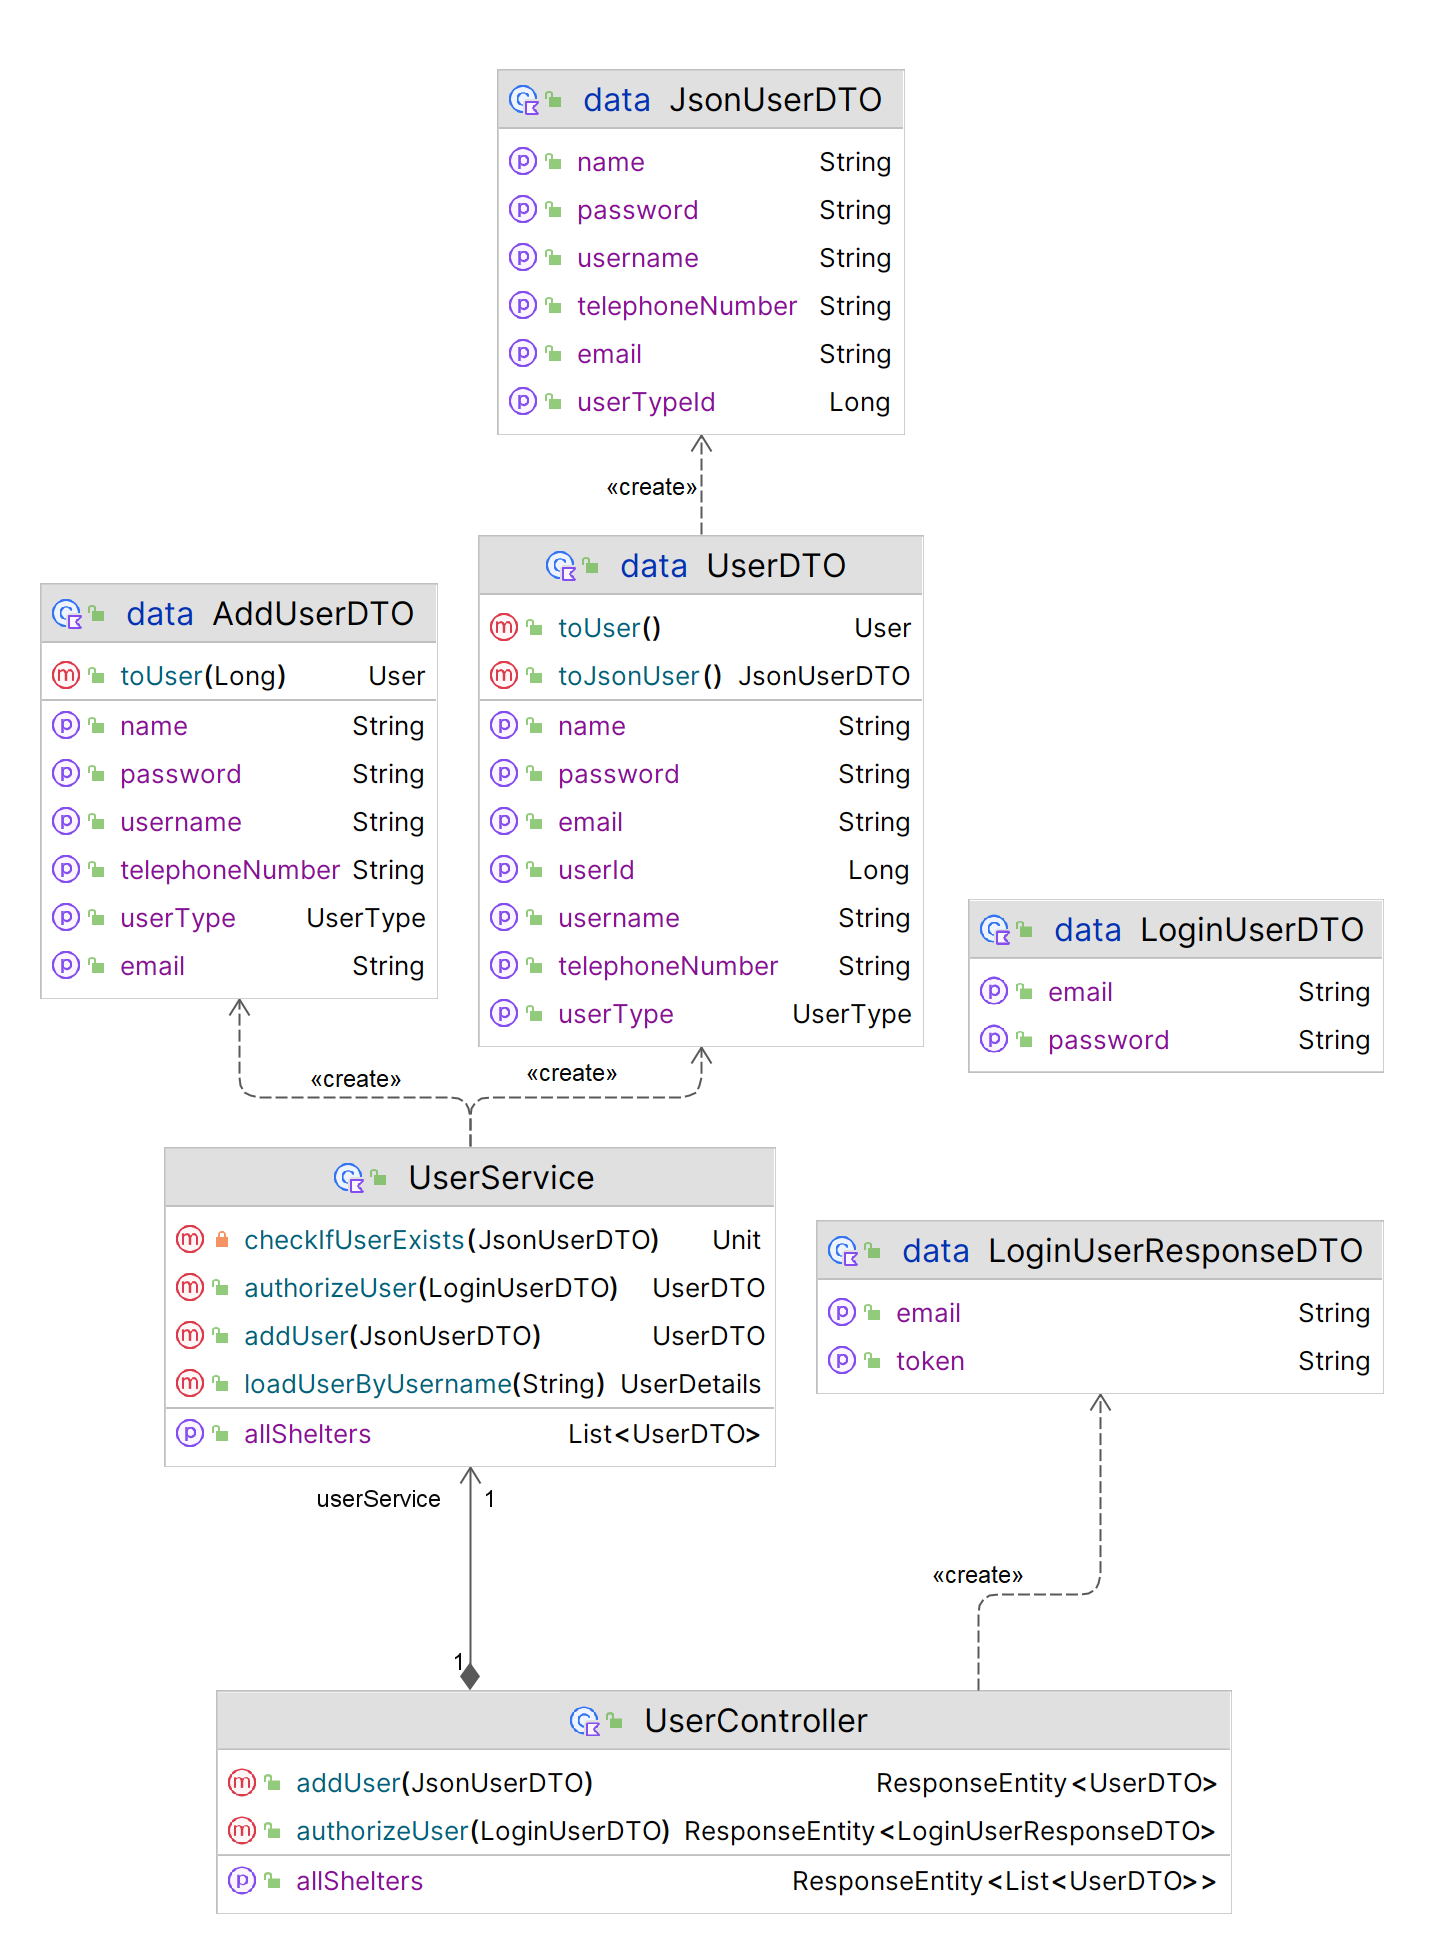
\includegraphics[scale=0.3]{slike/class_user.PNG} 
				\centering
				\caption{Razredi - korisnici}
				\label{class_user}
			\end{figure}
			
			\begin{figure}[H]
				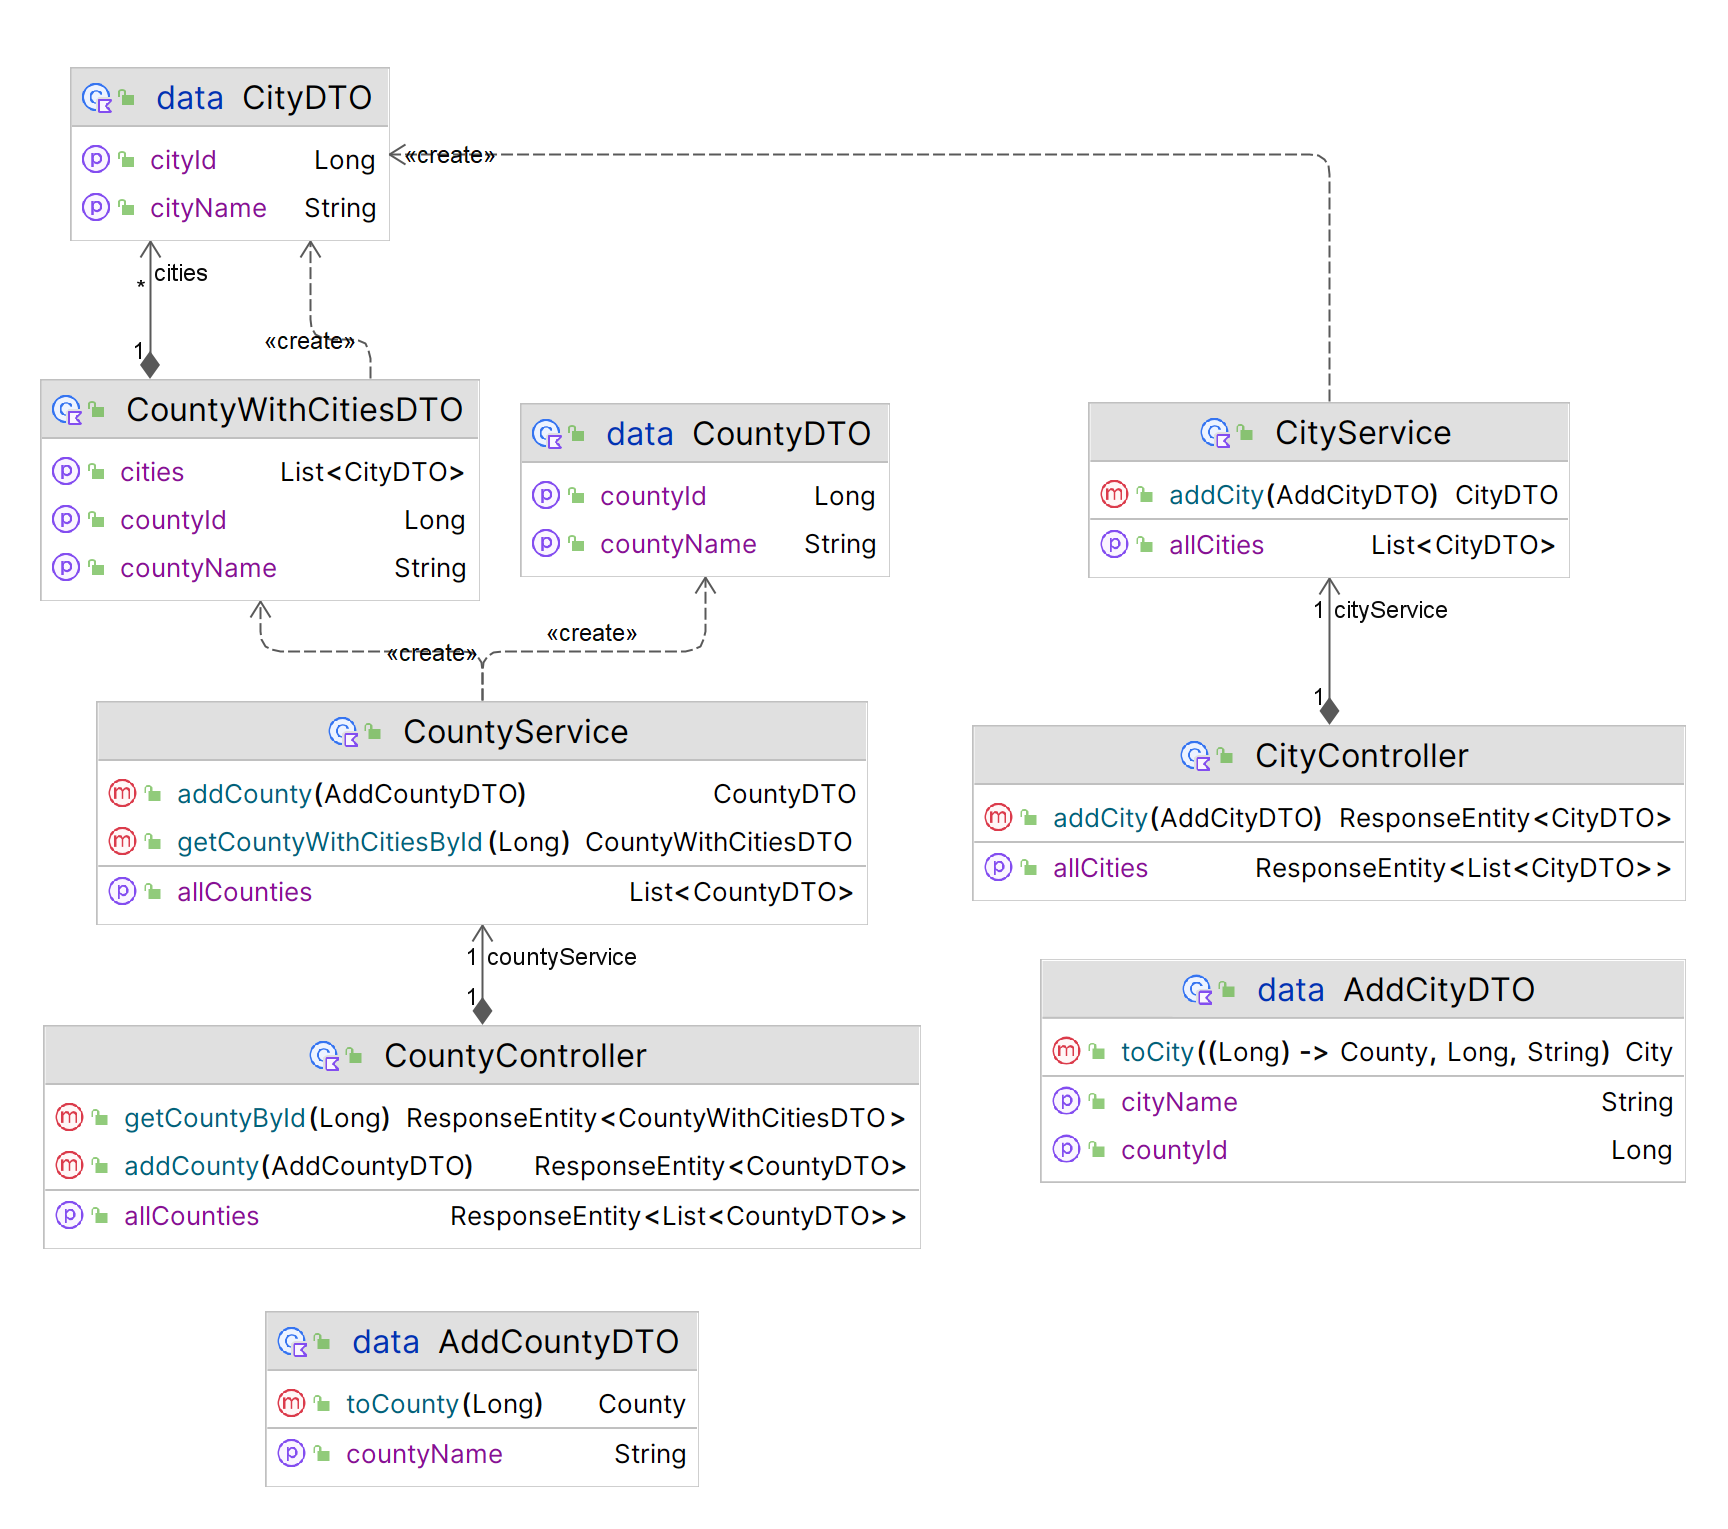
\includegraphics[scale=0.3]{slike/class_city_county.PNG} 
				\centering
				\caption{Razredi - gradovi i županije}
				\label{class_city_county}
			\end{figure}
			
			\begin{figure}[H]
				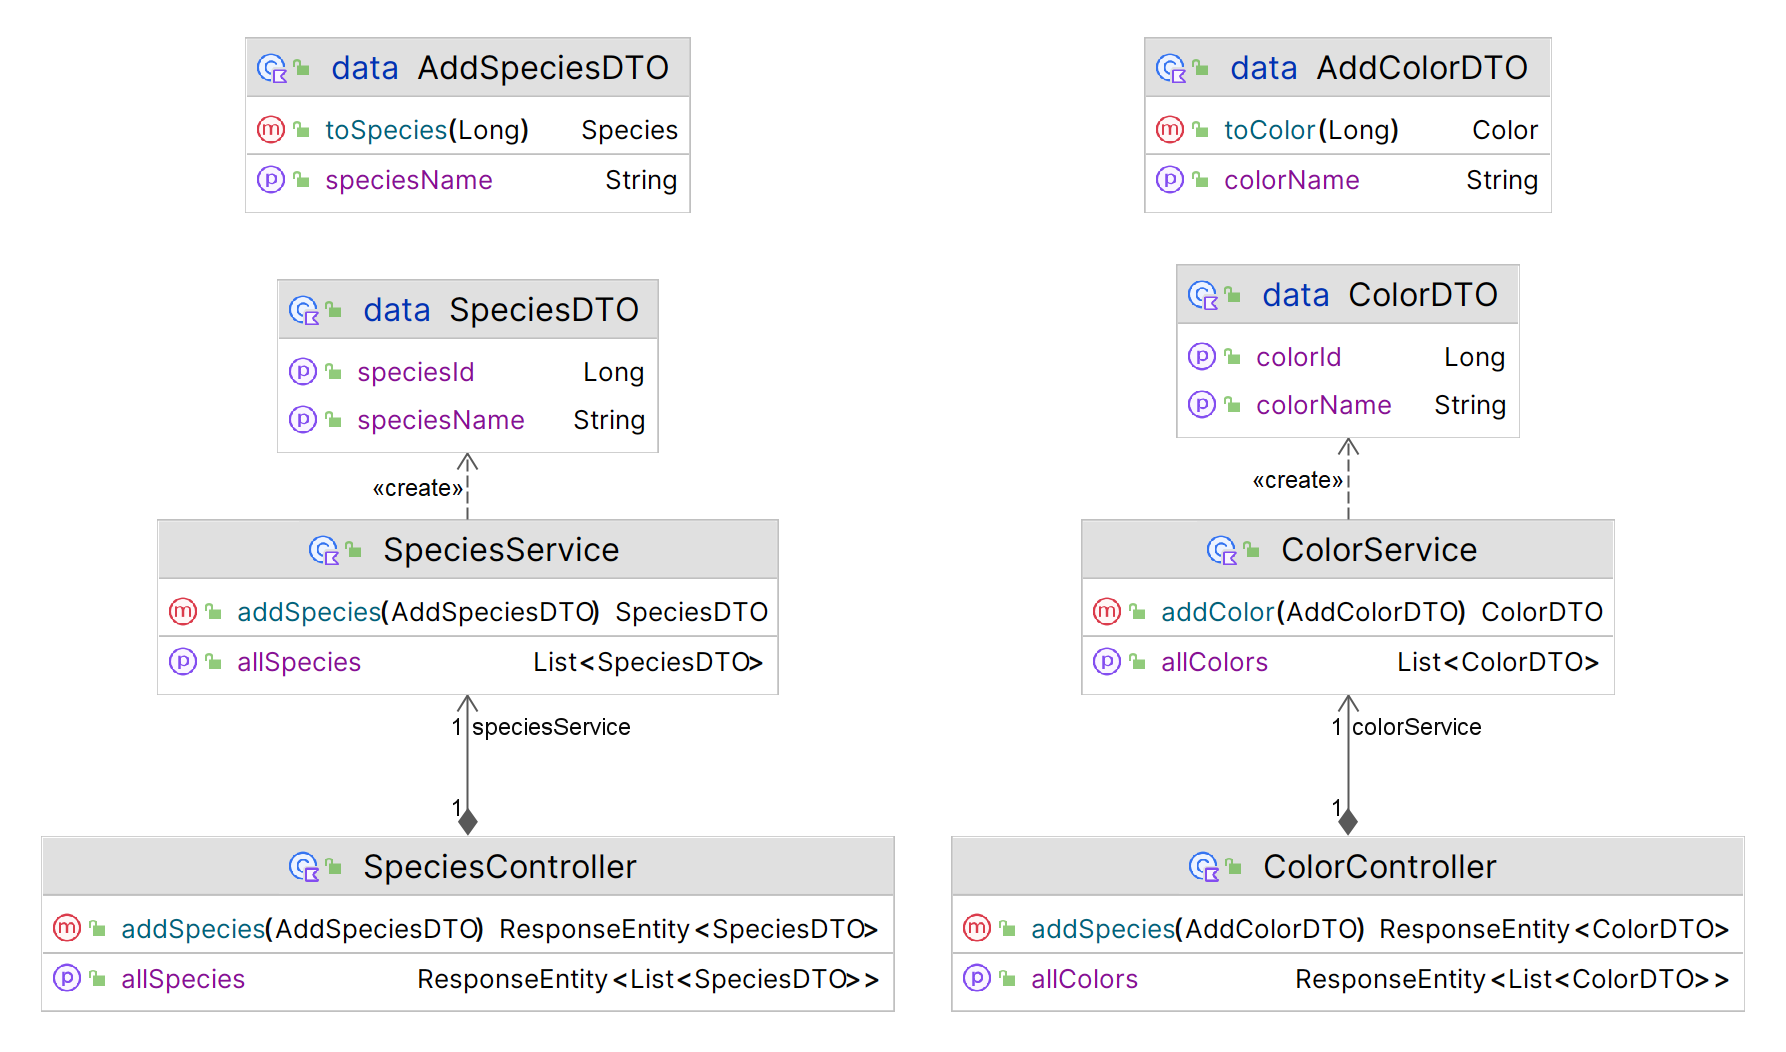
\includegraphics[scale=0.3]{slike/class_species_color.PNG} 
				\centering
				\caption{Razredi - vrste i boje ljubimaca}
				\label{class_species_color}
			\end{figure}
			
			Na slici \ref{class_security_exc_cors} prikazani su razredi odgovorni za autorizaciju, upravljanje iznimkama te \textit{cross-origin resource sharing (CORS)}.
			
			\begin{figure}[H]
				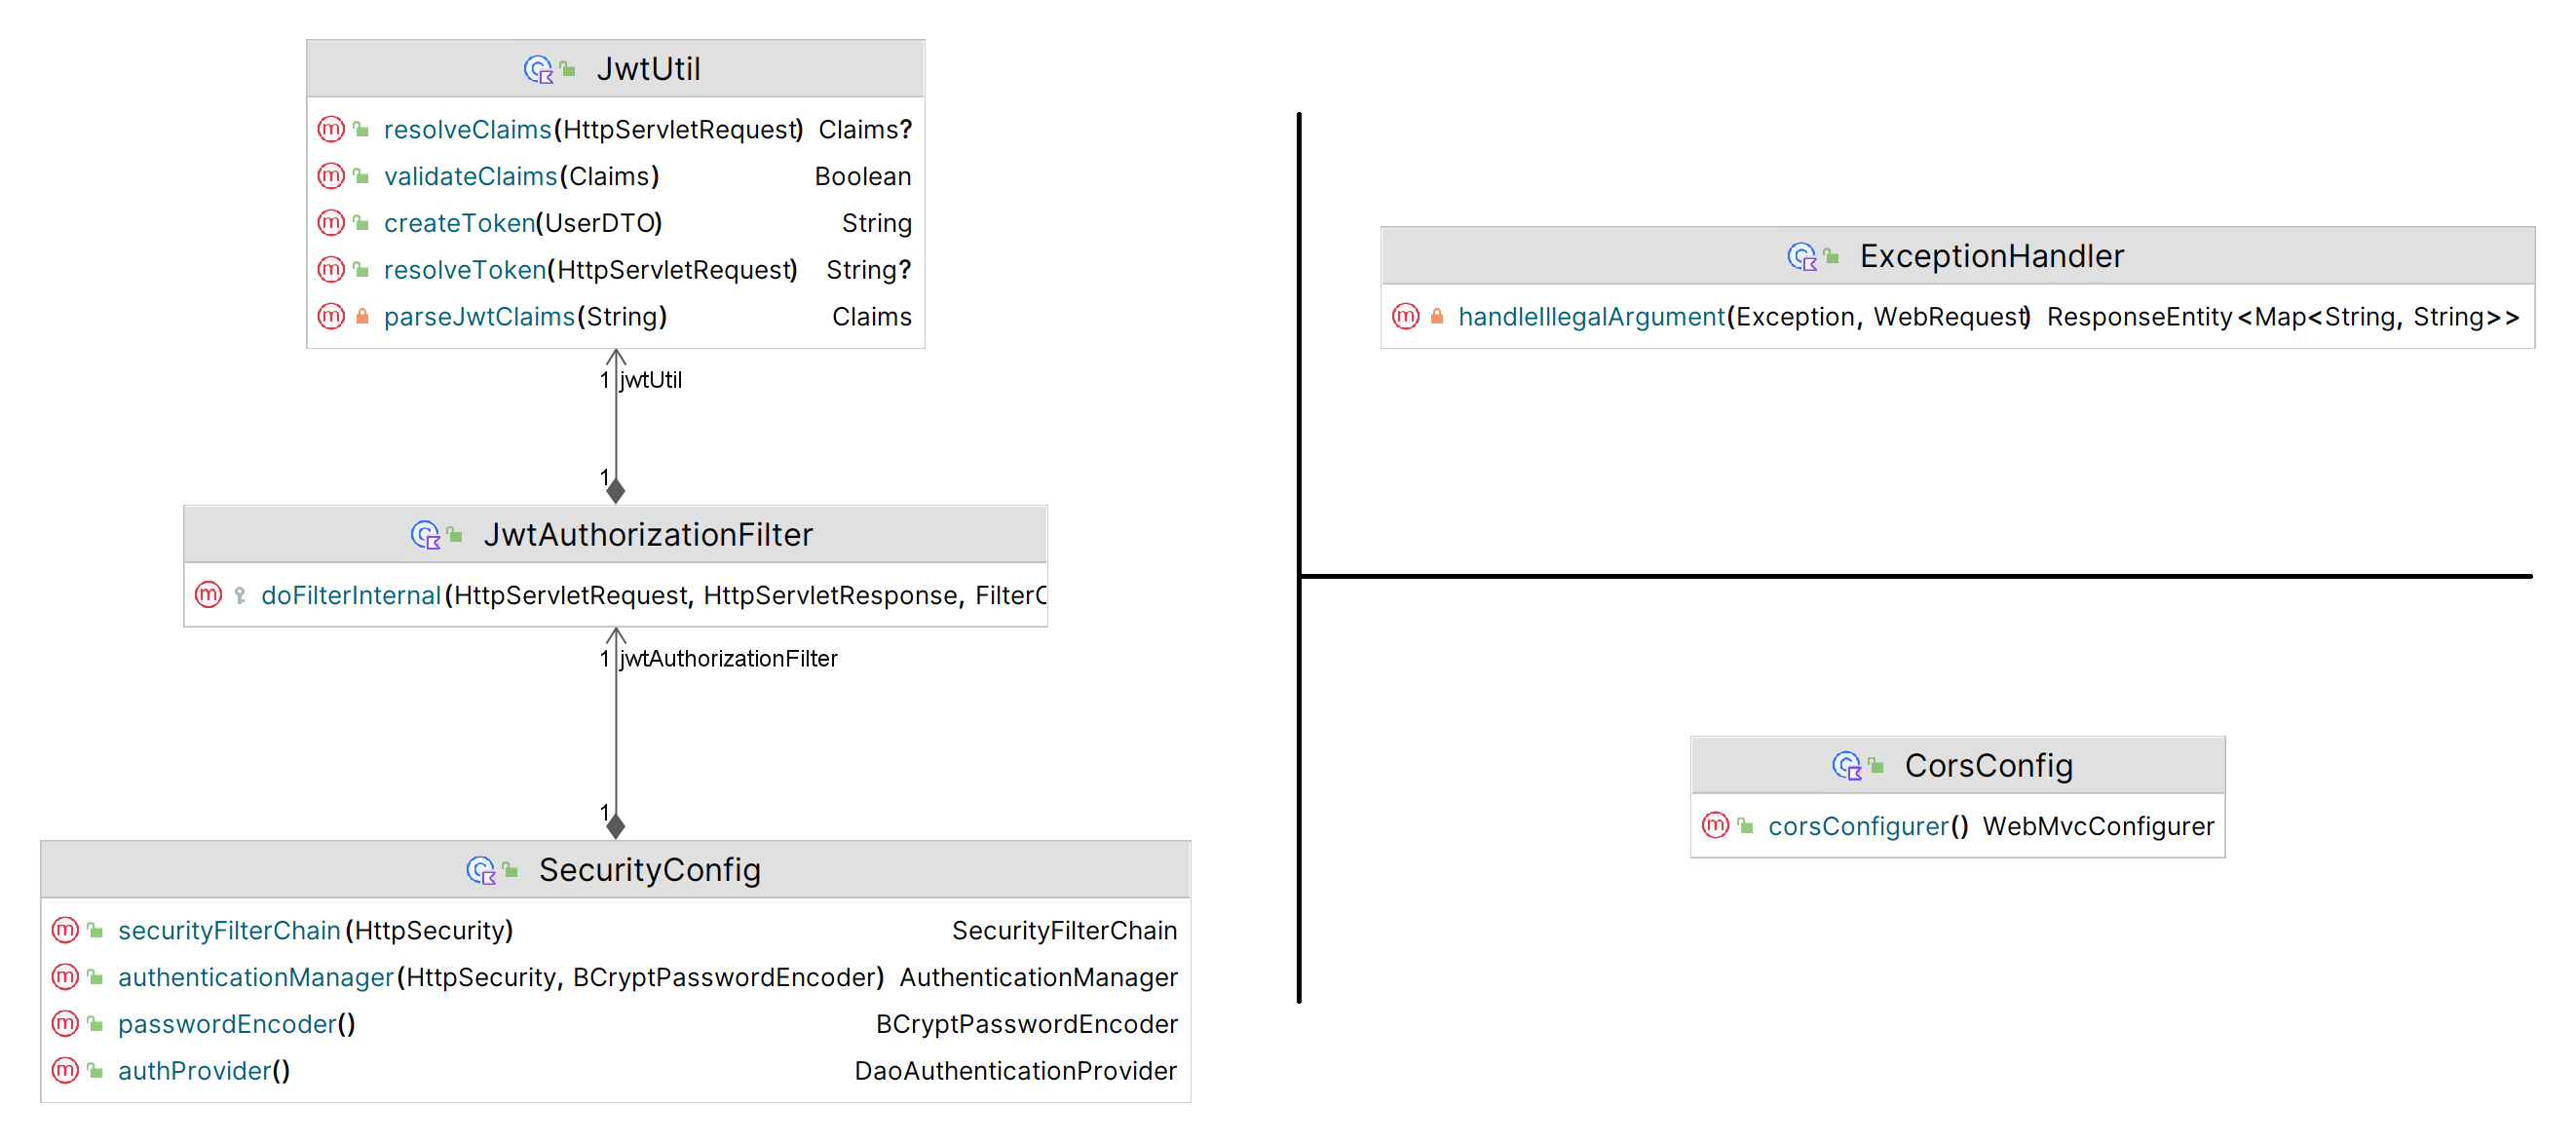
\includegraphics[scale=0.3]{slike/class_security_exc_cors.PNG} 
				\centering
				\caption{Autorizacija, upravljanje iznimkama i CORS}
				\label{class_security_exc_cors}
			\end{figure}
			
			\eject
		
		\section{Dijagram stanja}
			
			Slika \ref{dijagram_stanja} prikazuje dijagram stanja za prijavljenog korisnika. Nakon prijave, korisniku se prikazuje početna stranica na kojoj može vidjeti oglase o nestalim ljubimcima. Korisnik ima mogućnost pregledati detalje nekog oglasa, kao i kontakt podatke korisnika koji je objavio oglas te pregledati poruke i sudjelovati u komunikaciji slanjem vlastite poruke. Klik na "Shelters" vodi korisnika na prikaz popisa skloništa čije oglase zatim može pregledati (nazad se vraća klikom na "Posts"). Gumb s ikonicom "Account" prikazuje korisniku osobne podatke i postavljene oglase, koje korisnik može (klikom na "...") obrisati ili urediti (izmijeniti podatke, promijeniti kategoriju). Gumb "Post new ad" otvara formu za stvaranje novog oglasa. Klikom na gumb "Map" korisniku se prikazuje karta na kojoj su označene lokacije nestalih ljubimaca. Na njih se može kliknuti i vidjeti pojednostavljeni prikaz oglasa.
			
			\begin{figure}[H]
				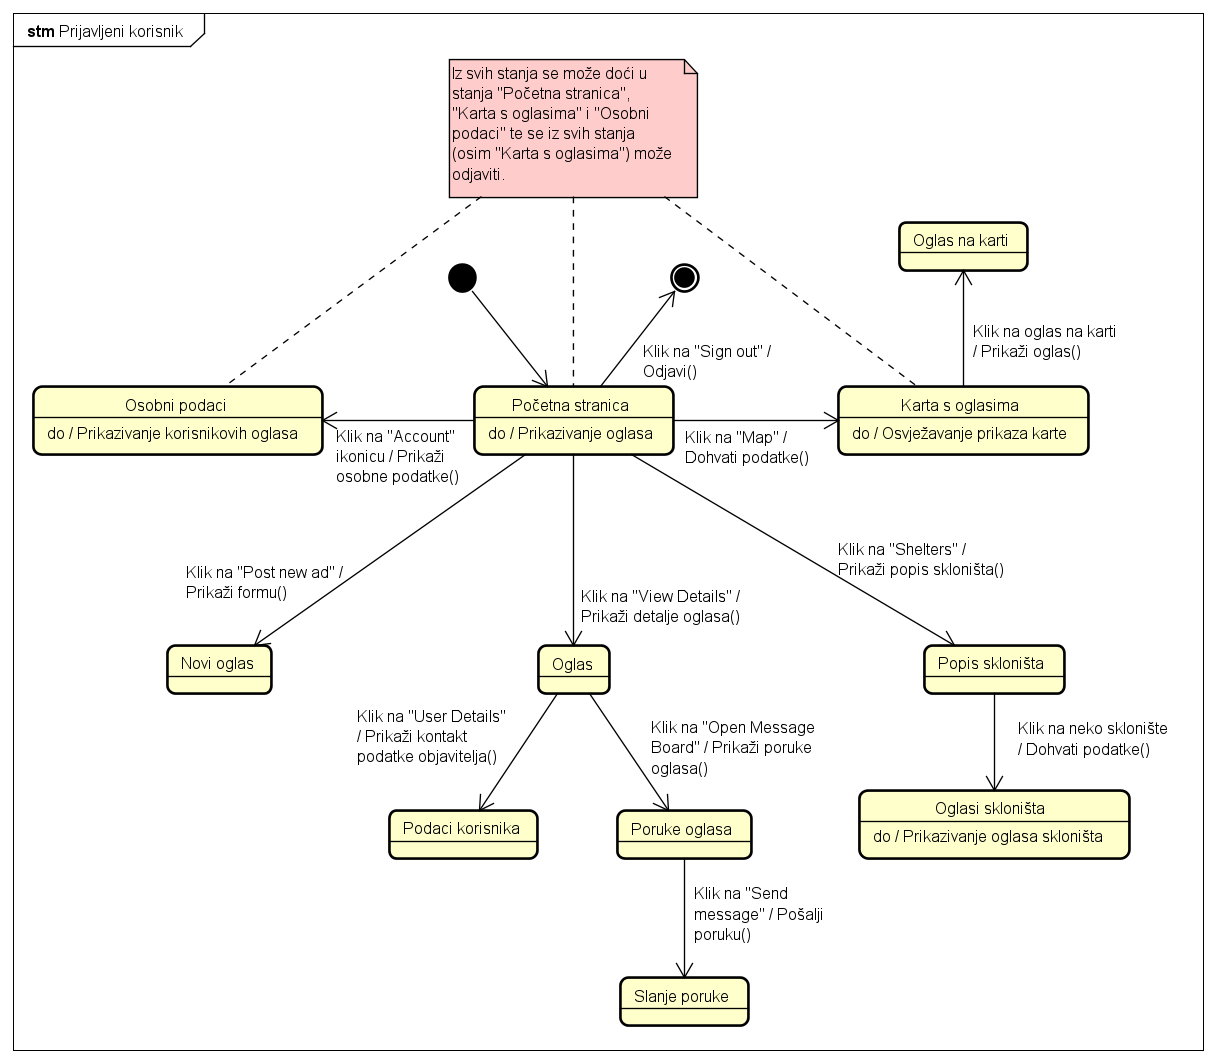
\includegraphics[scale=0.5]{slike/dijagram_stanja.PNG} 
				\centering
				\caption{Dijagram stanja}
				\label{dijagram_stanja}
			\end{figure}
			
			
			\eject 
		
		\section{Dijagram aktivnosti}
			
			Dijagram aktivnosti na slici \ref{dijagram_aktivnosti} prikazuje proces objave oglasa o nestalom ljubimcu. Korisnik se prijavi u sustav, odabere opciju stvaranja novog oglasa te ispunjava formu za oglas. Nakon što korisnik unese sve potrebne podatke i preda formu, oglas se pohranjuje u bazu podataka te se korisnika vraća na početnu stranicu.
			 
			 \begin{figure}[H]
				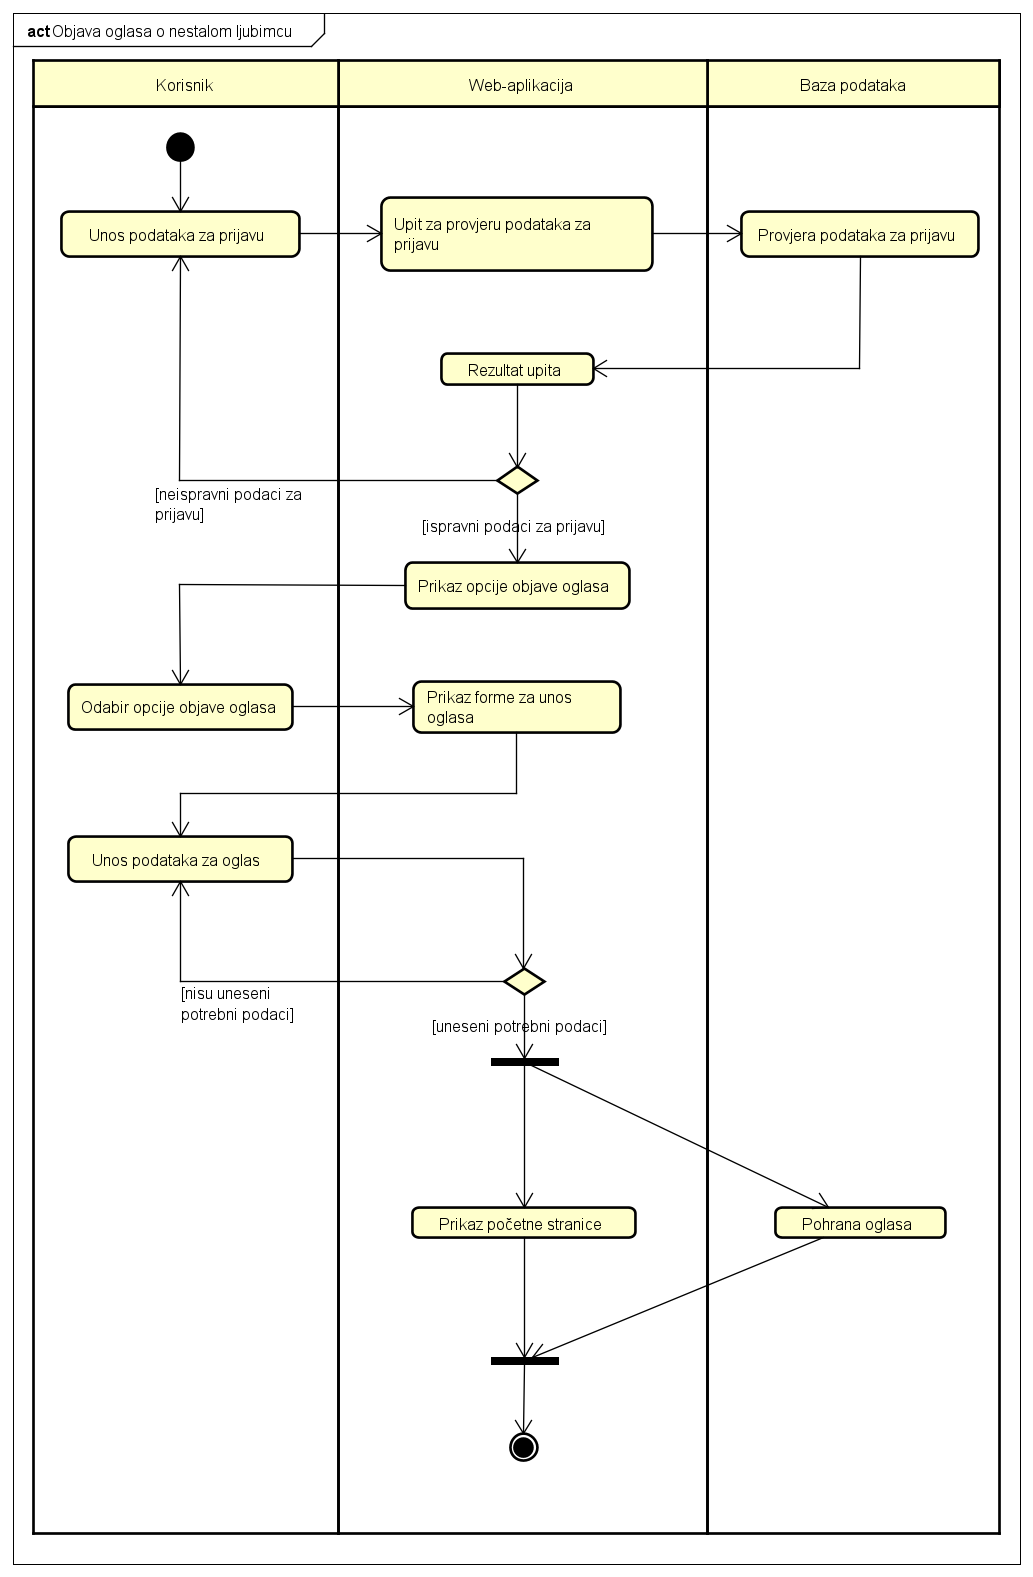
\includegraphics[scale=0.5]{slike/dijagram_aktivnosti.PNG} 
				\centering
				\caption{Dijagram aktivnosti}
				\label{dijagram_aktivnosti}
			\end{figure}
			
			\eject
		
		\section{Dijagram komponenti}
		
			Dijagram komponenti na slici \ref{dijagram_komponenti} prikazuje ustroj i međuovisnost komponenti, interne strukture i odnose prema okolini. Dva su sučelja putem kojih se pristupa sustavu. Sučelje za dohvat CSS, JS i TS datoteka odgovorno je za posluživanje datoteka vezanih uz \textit{frontend}. Sve TS odnosno JS datoteke ovise o React biblioteci. Sučeljem za dohvat JSON podataka se pristupa REST API komponenti, odgovornoj za posluživanje podataka vezanih uz \textit{backend}. Tablice se iz baze podataka dohvaćaju pomoću JPA (\textit{Jakarta Persistence}). Podaci iz baze se prosljeđuju kao DTO (\textit{data transfer object}).
			 
			 \begin{figure}[H]
				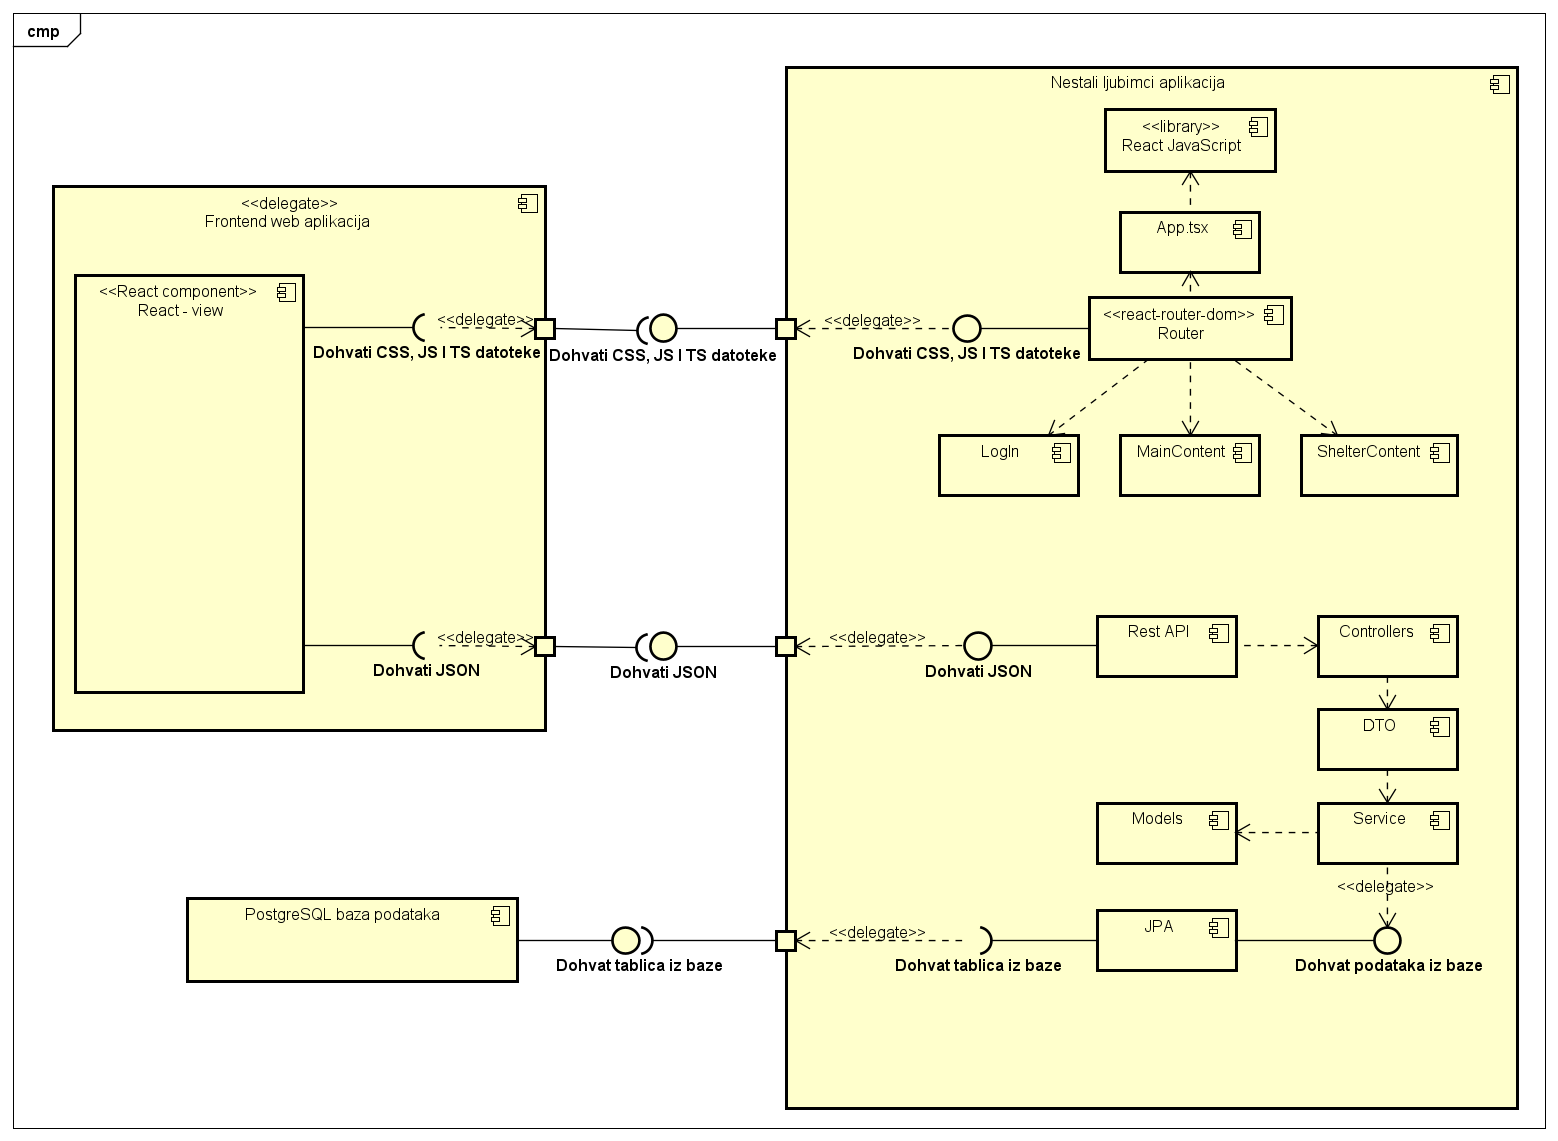
\includegraphics[scale=0.4]{slike/dijagram_komponenti.PNG} 
				\centering
				\caption{Dijagram komponenti}
				\label{dijagram_komponenti}
			\end{figure}